\section{Experiments}
There are a number of different axes on which we can evaluate \sys.
First, we take real datasets and generate various types of errors to illustrate the value of data cleaning in comparison to robust statistical techniques.
Next, we explore different prioritization and model update schemes for data cleaning samples.
Finally, we evaluate \sys end-to-end in a number of real-world data cleaning scenarios.

\subsection{Experimental Setup and Notation}
Every experiment has two steps: data cleaning and model evaluation.
We evaluate the data cleaning on one metric:

\vspace{0.5em}

\noindent\textbf{Cleaning Efficiency. } Let $K$ be the number of samples processed by the algorithm, and $K'$ be the number of samples that were actually dirty. 
The cleaning efficiency is $\frac{K'}{K}$.
In our experiments, we explore three classification models: L1-Hinge Loss SVM, Logistic Regression, and Thresholded Linear Regression.
We evaluate the trained models on the following metrics:

\vspace{0.5em}

\noindent\textbf{Relative Model Error. } Let $\theta$ be the model trained on the dirty data, and let $\theta^*$ be the model trained on the same data if it was cleaned. Then the model error is defined as $\frac{\|\theta - \theta^*\|}{\|\theta^*\|}$.

\vspace{0.5em}

\noindent\textbf{Testing Accuracy. } Let $\theta$ be the model trained on the dirty data, and let $\theta^*$ be the model trained on the same data if it was cleaned. Let $T(\theta)$ be the out-of-sample testing accuracy when the dirty model is applied to the clean data, and $T(\theta^*)$ be the testing accuracy when the clean model is applied to the clean data. The testing error is defined as $T(\theta^*) - T(\theta)$

\subsubsection{Scenarios}
We apply these models in the following scenarios:

\vspace{0.5em}

\noindent\textbf{Housing: } In this dataset, our task is to predict housing prices from 13 numerical and categorical covariates. There are 550 data points in this dataset. The model is a Logistic Regression classifier which predicts if the house price is greater than \$500k.

\vspace{0.5em}

\noindent\textbf{Adult: } In this census dataset, our task is to predict the income bracket (binary) from 12 numerical and categorical covariates. There are 45552 data points in this dataset. We use a SVM classifier to predict the income bracket of the person.

\vspace{0.5em}

\noindent\textbf{EEG: } In this dataset, our task is to predict the on set of a seizure (binary) from 15 numerical covariates. There are 14980 data points in this dataset. This dataset is unique because the classification is hard with linear predictors. The model that we use is a thresholded Linear Regression.

\vspace{0.5em}

\noindent\textbf{MNIST: } In this dataset, our task is to classify 60,000 images of handwritten images into 10 categories. The unique part of this dataset is the featurized data consists of a 784 dimensional vector which includes edge detectors and raw image patches. We use this dataset to explore how we can corrupt the raw data to affect subsequent featurization. The model is an one-to-all multiclass SVM classifier. 

\subsubsection{Alternative Algorithms}
Here are the alternative methodologies that we consider:

\vspace{0.5em}

\noindent\textbf{Robust Logistic Regression \cite{feng2014robust}. } Feng et al. proposed a variant of logistic regression that is robust to outliers. 

\vspace{0.5em}

\noindent\textbf{Discarding Dirty Data \cite{li2014improved}. } A methodology that has shown suprising empirical success in secure Machine Learning is rejection-on-negative-impact. In this model, data that negatively affects the loss is discarded.

\vspace{0.5em}

\noindent\textbf{SampleClean (SC) \cite{wang1999sample}. } In SampleClean, we take a sample of data, apply data cleaning, and then train a model to completion.

\vspace{0.5em}

\noindent\textbf{Active Learning (AL) \cite{guillory2009active}. } There have been recent proposals of integrating Active Learning with stochastic optimization. Active Learning has been widely applied in the data cleaning literature \cite{gokhale2014corleone}, but never integrated with model training. We acknowledge the work in the Machine Learning literature and formulate an Active Learning that uses a prioritization fuction agnostic of the dirty data (no error impact estimates and partitioning). 

\vspace{0.5em}

\noindent\textbf{ActiveClean Oracle (AC+O): } In \sys Oracle, we importance sample points by their clean gradient. This represents the theoretical best that our algorithm could hope to achieve given perfect error estimation.

\subsection{Experiment 1. Effect of Cleaning}
Before we evaluate \sys, we first evaluate the benefits of cleaning on our 4 example datasets.
We first explore this problem without sampling to understand which types of errors are amenable to data cleaning and which are better suited for robust statistical techniques.
We compare 4 schemes: (1) full data cleaning, (2) robust logistic regression, (3) discarding the dirty data, and (4) baseline of no cleaning. We corrupted 5\% of the training examples in each dataset in two different ways:

\vspace{0.5em}

\noindent\textbf{Random errors: } We simulated high-magnitude random outliers. We select 5\% of the examples and features uniformly at random and replace a feature with 3 times the highest feature value.

\vspace{0.5em}

\noindent\textbf{Systematic errors: } We simulated innocuous looking (but still incorrect) systematic errors. We trained the model on the clean data, find the most important feature (highest weighted). We sort examples but this feature and corrupt the top 5\% of examples with the mean value for that feature.

\begin{figure}[ht!]
\centering
 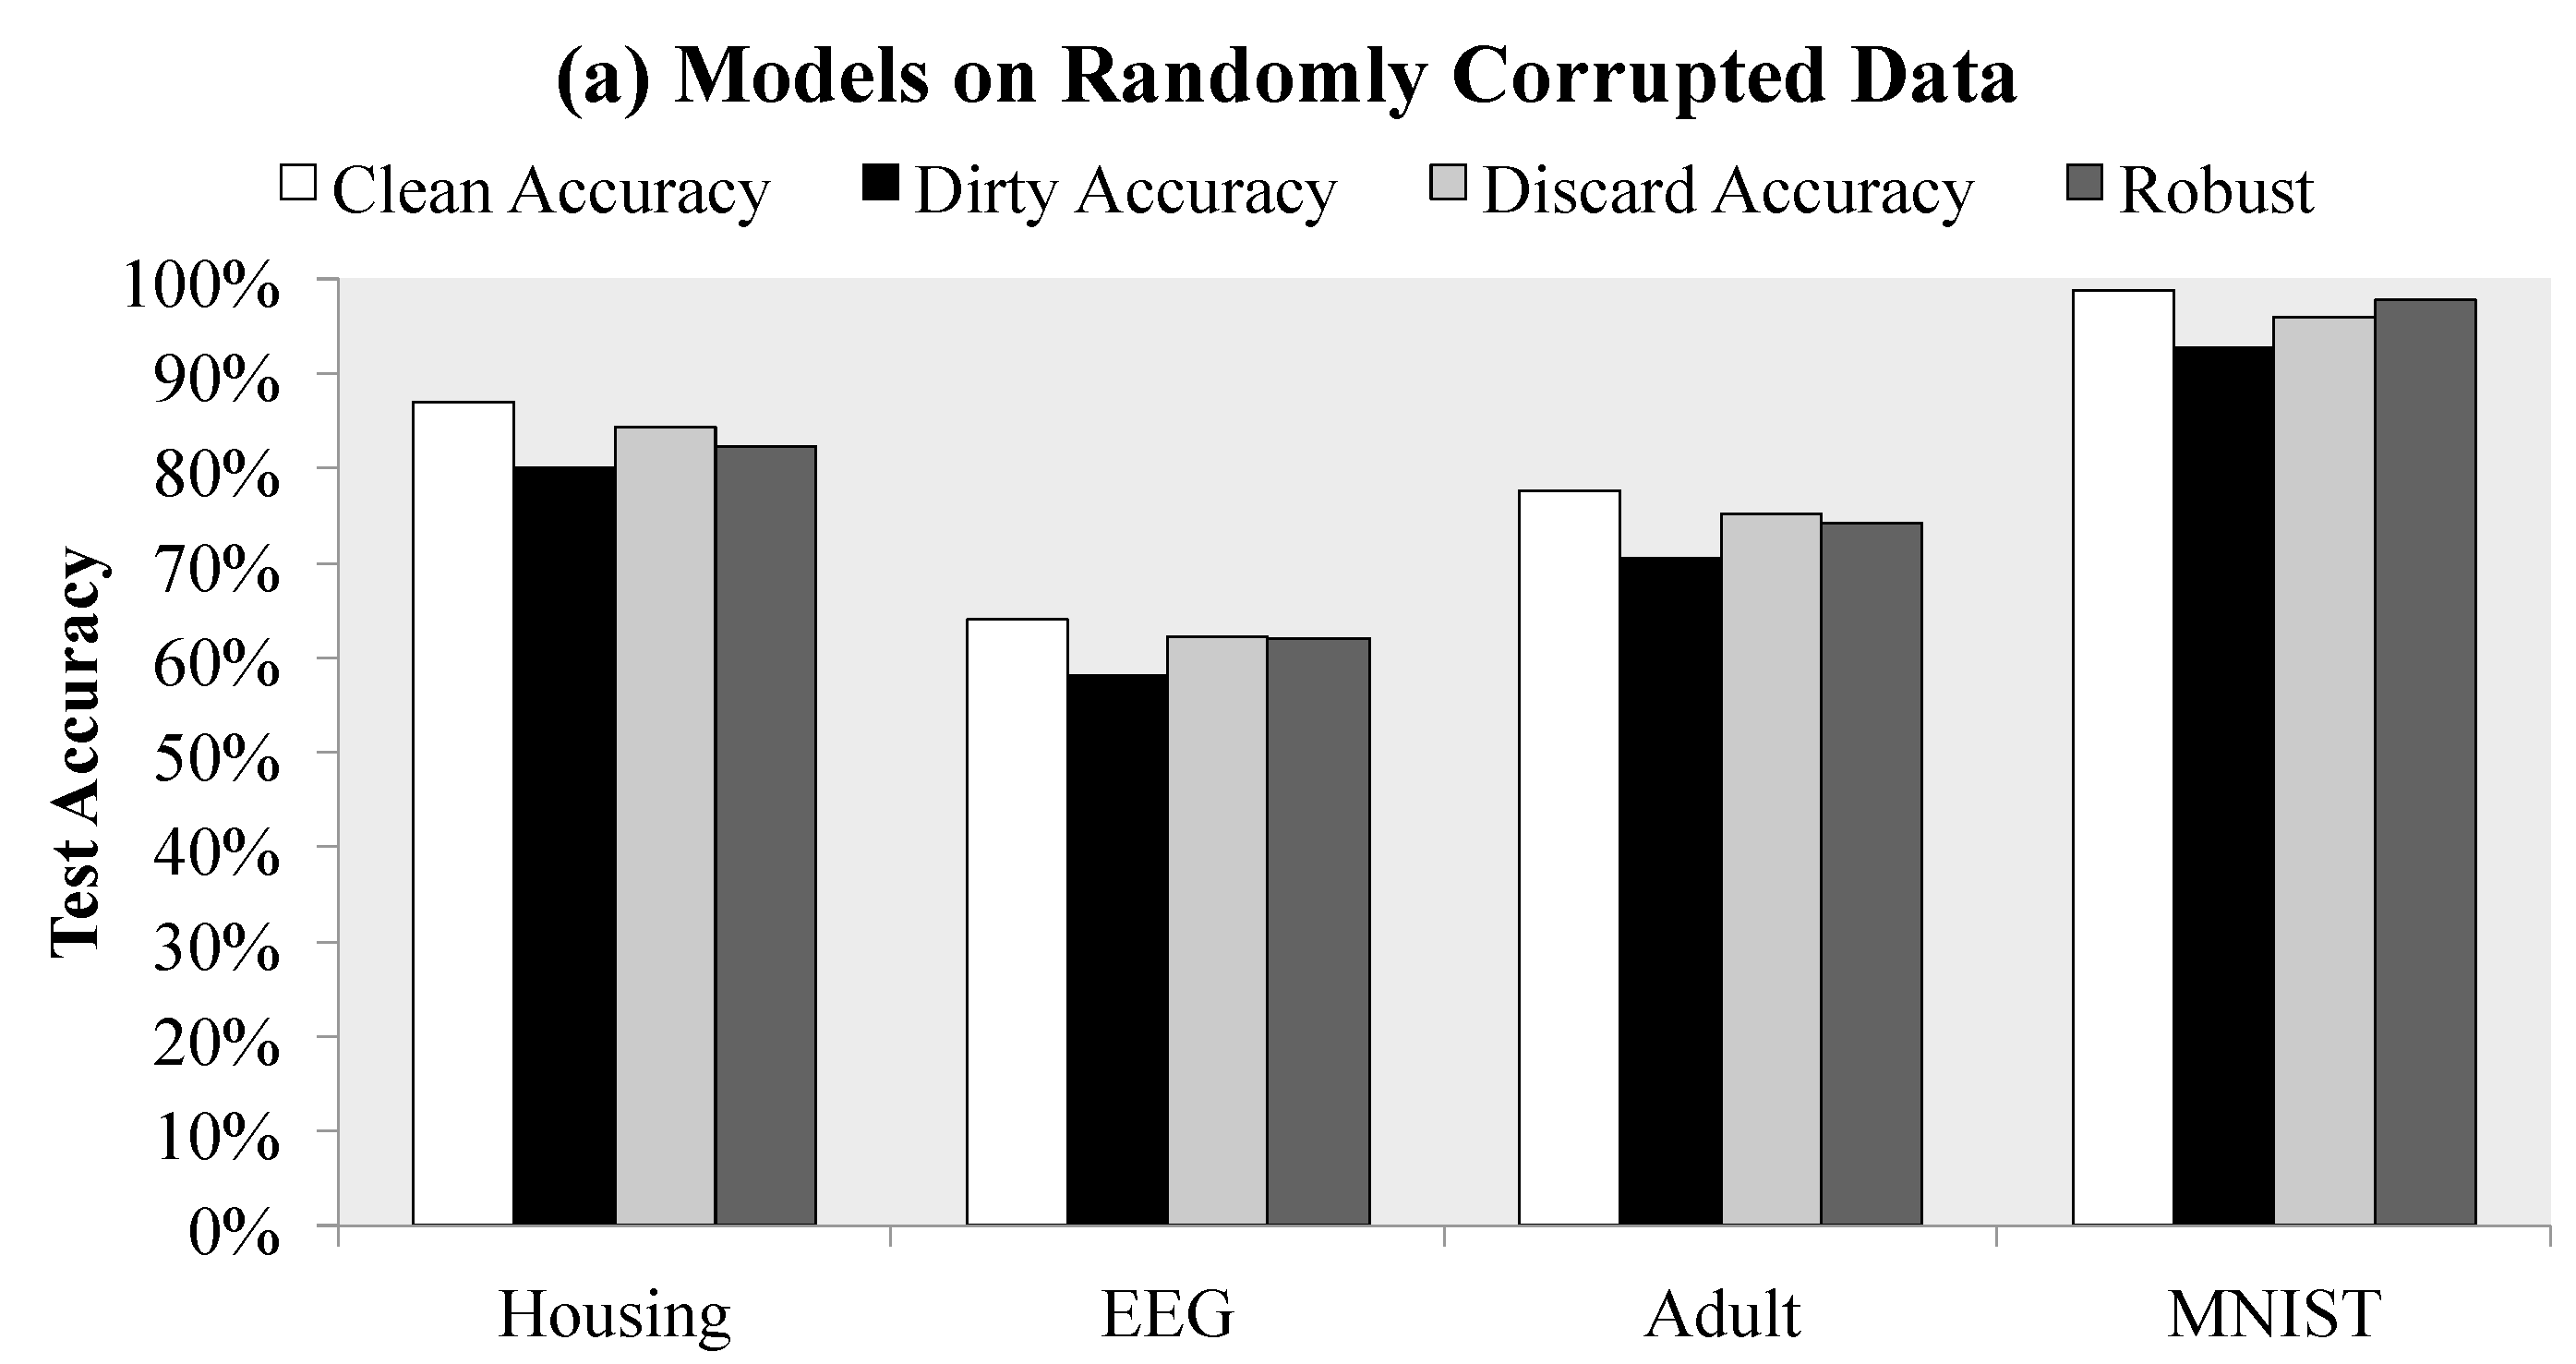
\includegraphics[width=\columnwidth]{exp/exp2.pdf}
 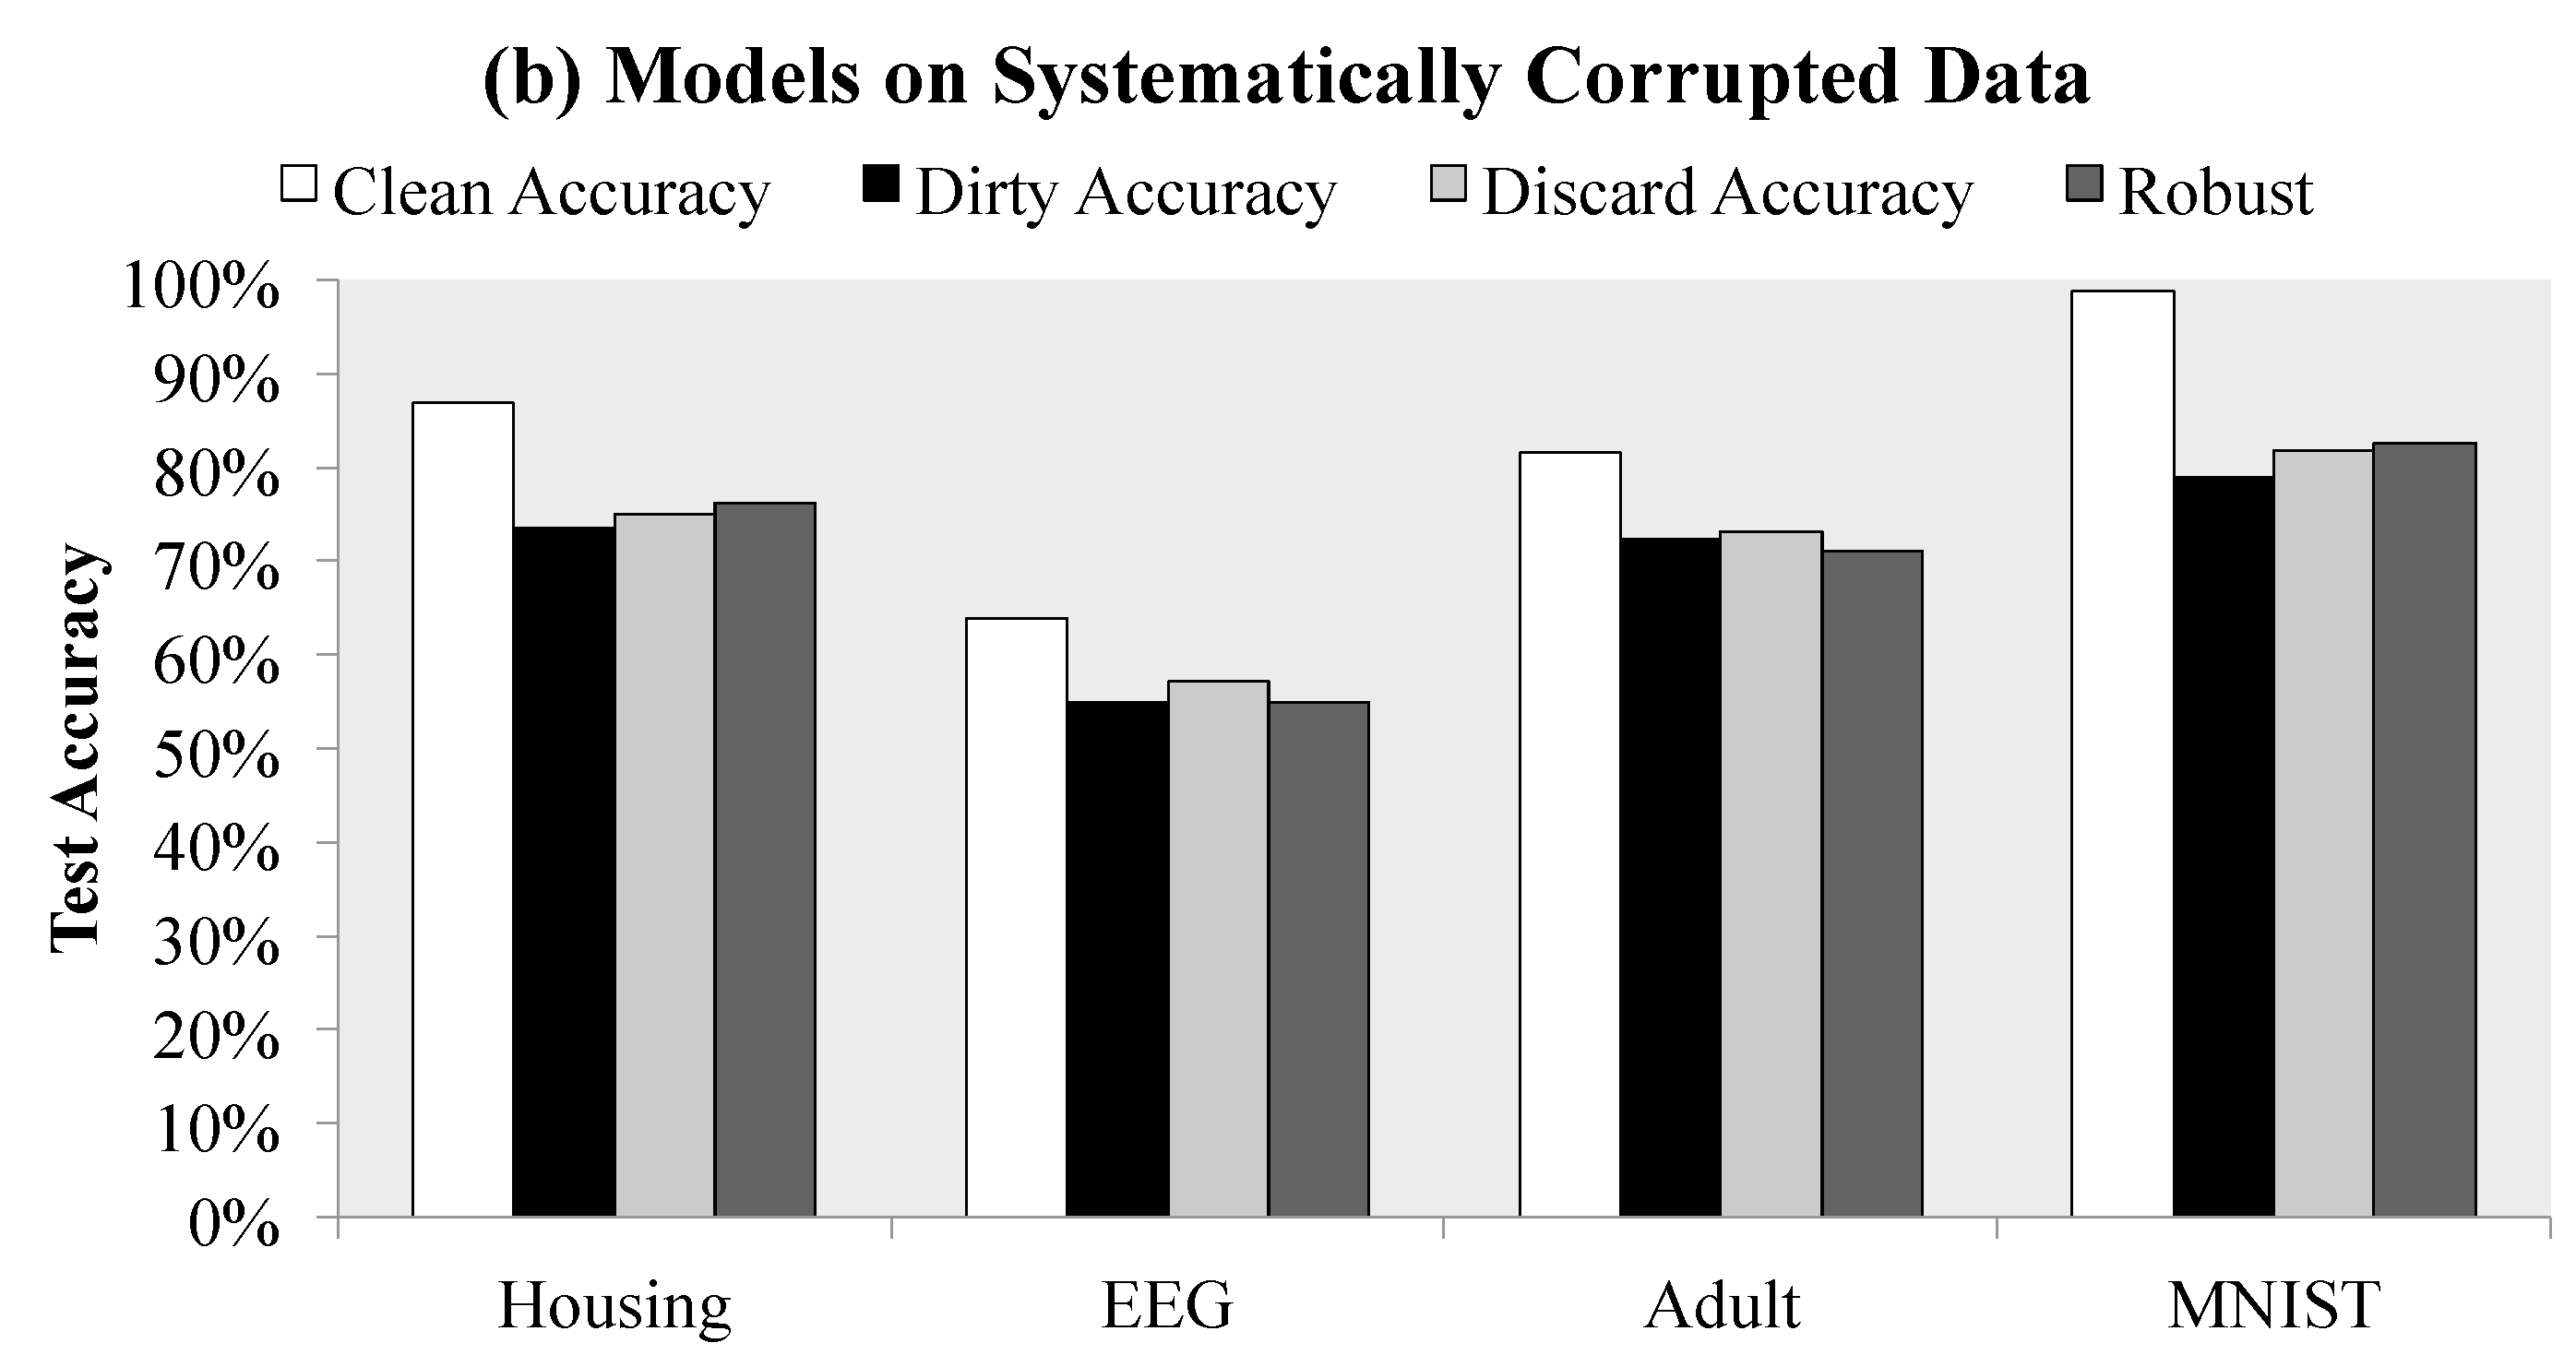
\includegraphics[width=\columnwidth]{exp/exp1.pdf}
 \caption{(a) Robust techniques work best when corrupted data are random and look atypical. (b)Data cleaning can provide reliable performance in both the systematically corrupted setting and randomly corrupted setting.\label{sys-rand}}
\end{figure}

In Figure \ref{sys-rand}, we present the results of this experiment.
As we argued in this paper, the robust method performs well on the random high-magnitude outliers, however, falters on the systematic corruption.
Interestingly enough, in the random setting, discarding dirty data also performs well.
However, when errors are systematic data cleaning is the most reliable option across datasets.
In the MNIST dataset, we see a particularly significant effect of systematic corruption
where the test accuracy drops from nearly 98\% to 78\%.
Multiclass classification is particularly sensitive to systematic corruption when the corruptions can make classes ambiguous (e.g. reconizing a ``4" and a ``9").
The problem is that a priori, we do not know if data error is random or systematic.
While data cleaning requires more effort, it provides benefits in both settings.

\subsection{Experiment 2. Prioritization}
The next set of experiments evaluate different approaches to cleaning a sample of data.
In this set of experiments, we generate errors in the following way: We select 5\% of the examples at random, then we corrupt the most informative feature by replacing it with 3 times the highest feature value.

\subsubsection{2a. Alternative Algorithms}
In our first prioritization experiment, we evaluate the samples-to-error tradeoff between three alternative algorithms: \sys, SampleClean, and Active Learning.
In Figure \ref{prio-perf}, we present our results on Housing, Adult, and EEG. 
We find that \sys gives its largest benefits for small sample sizes (up-to 12x).
\sys makes significant progress because of its intelligent initialization, iterative updates, and partitioning.
For example, the EEG dataset is the hardest classification task.
SampleClean has difficulty on this dataset since it takes a uniform sample of data (only 5\% of which are corrupted on average) and tries to train a model using only this data.
\sys and Active Learning leverage the initialization from the dirty data to get an improved result. 
However, \sys's impact estimates and error partitioning allow us to beat Active Learning on all three of the datasets.

\begin{figure*}[t]
\centering
 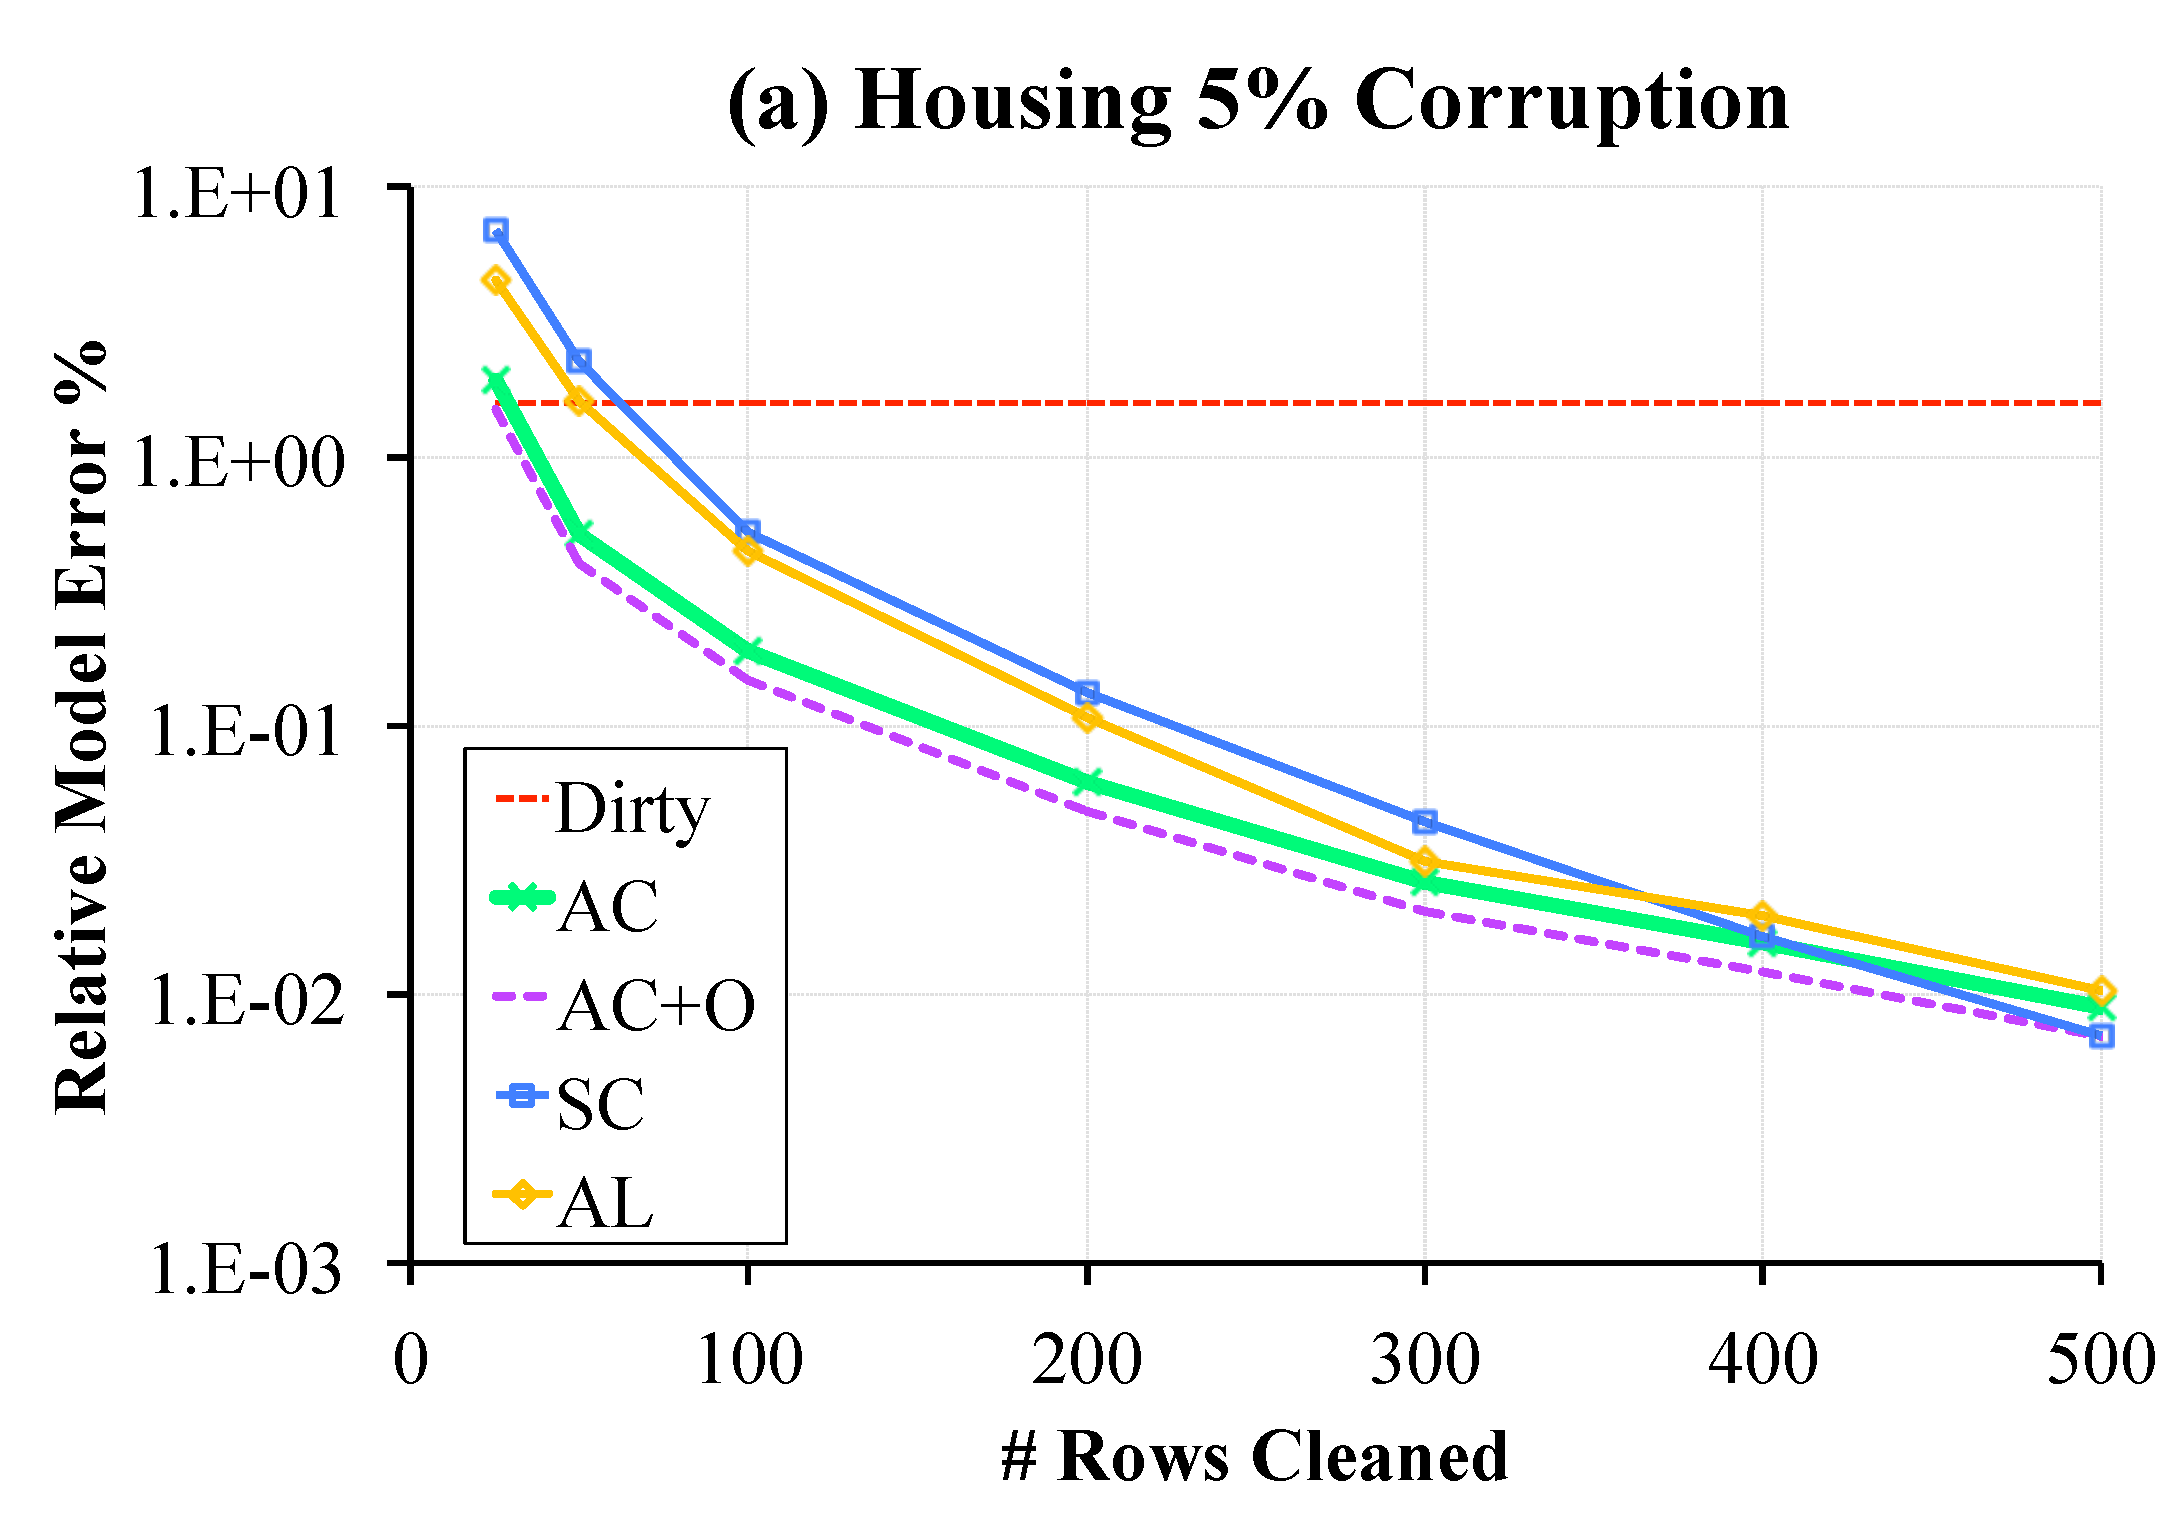
\includegraphics[scale=0.15]{exp/exp3a.pdf}
 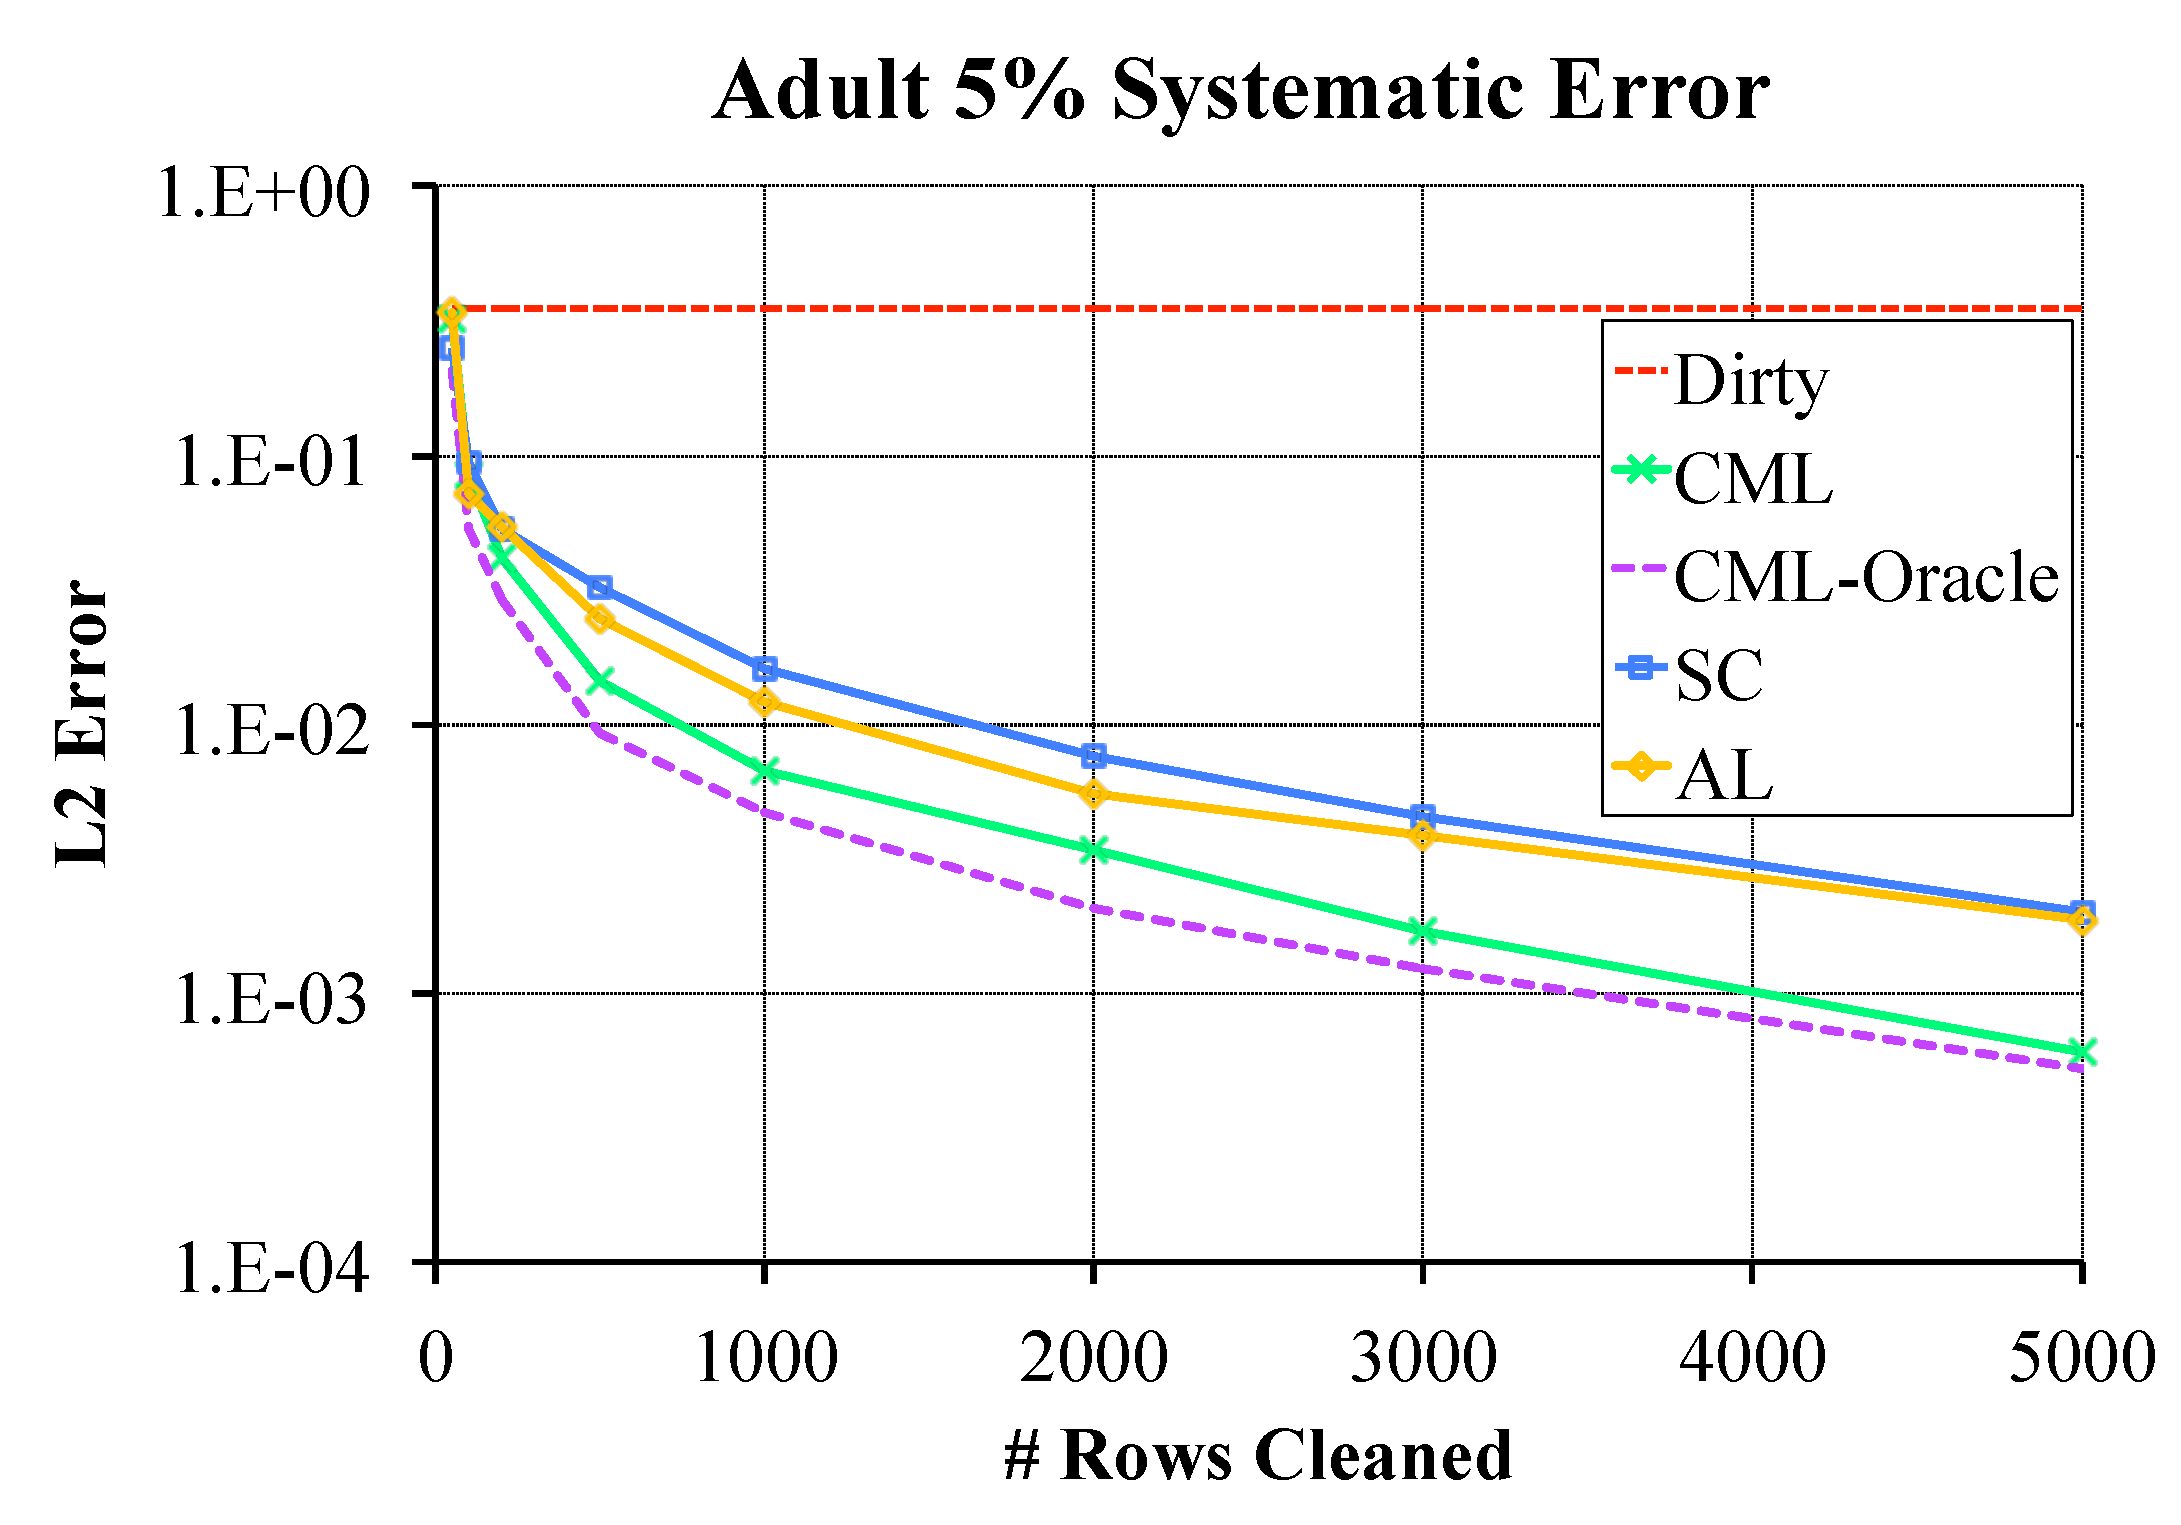
\includegraphics[scale=0.15]{exp/exp3b.pdf}
  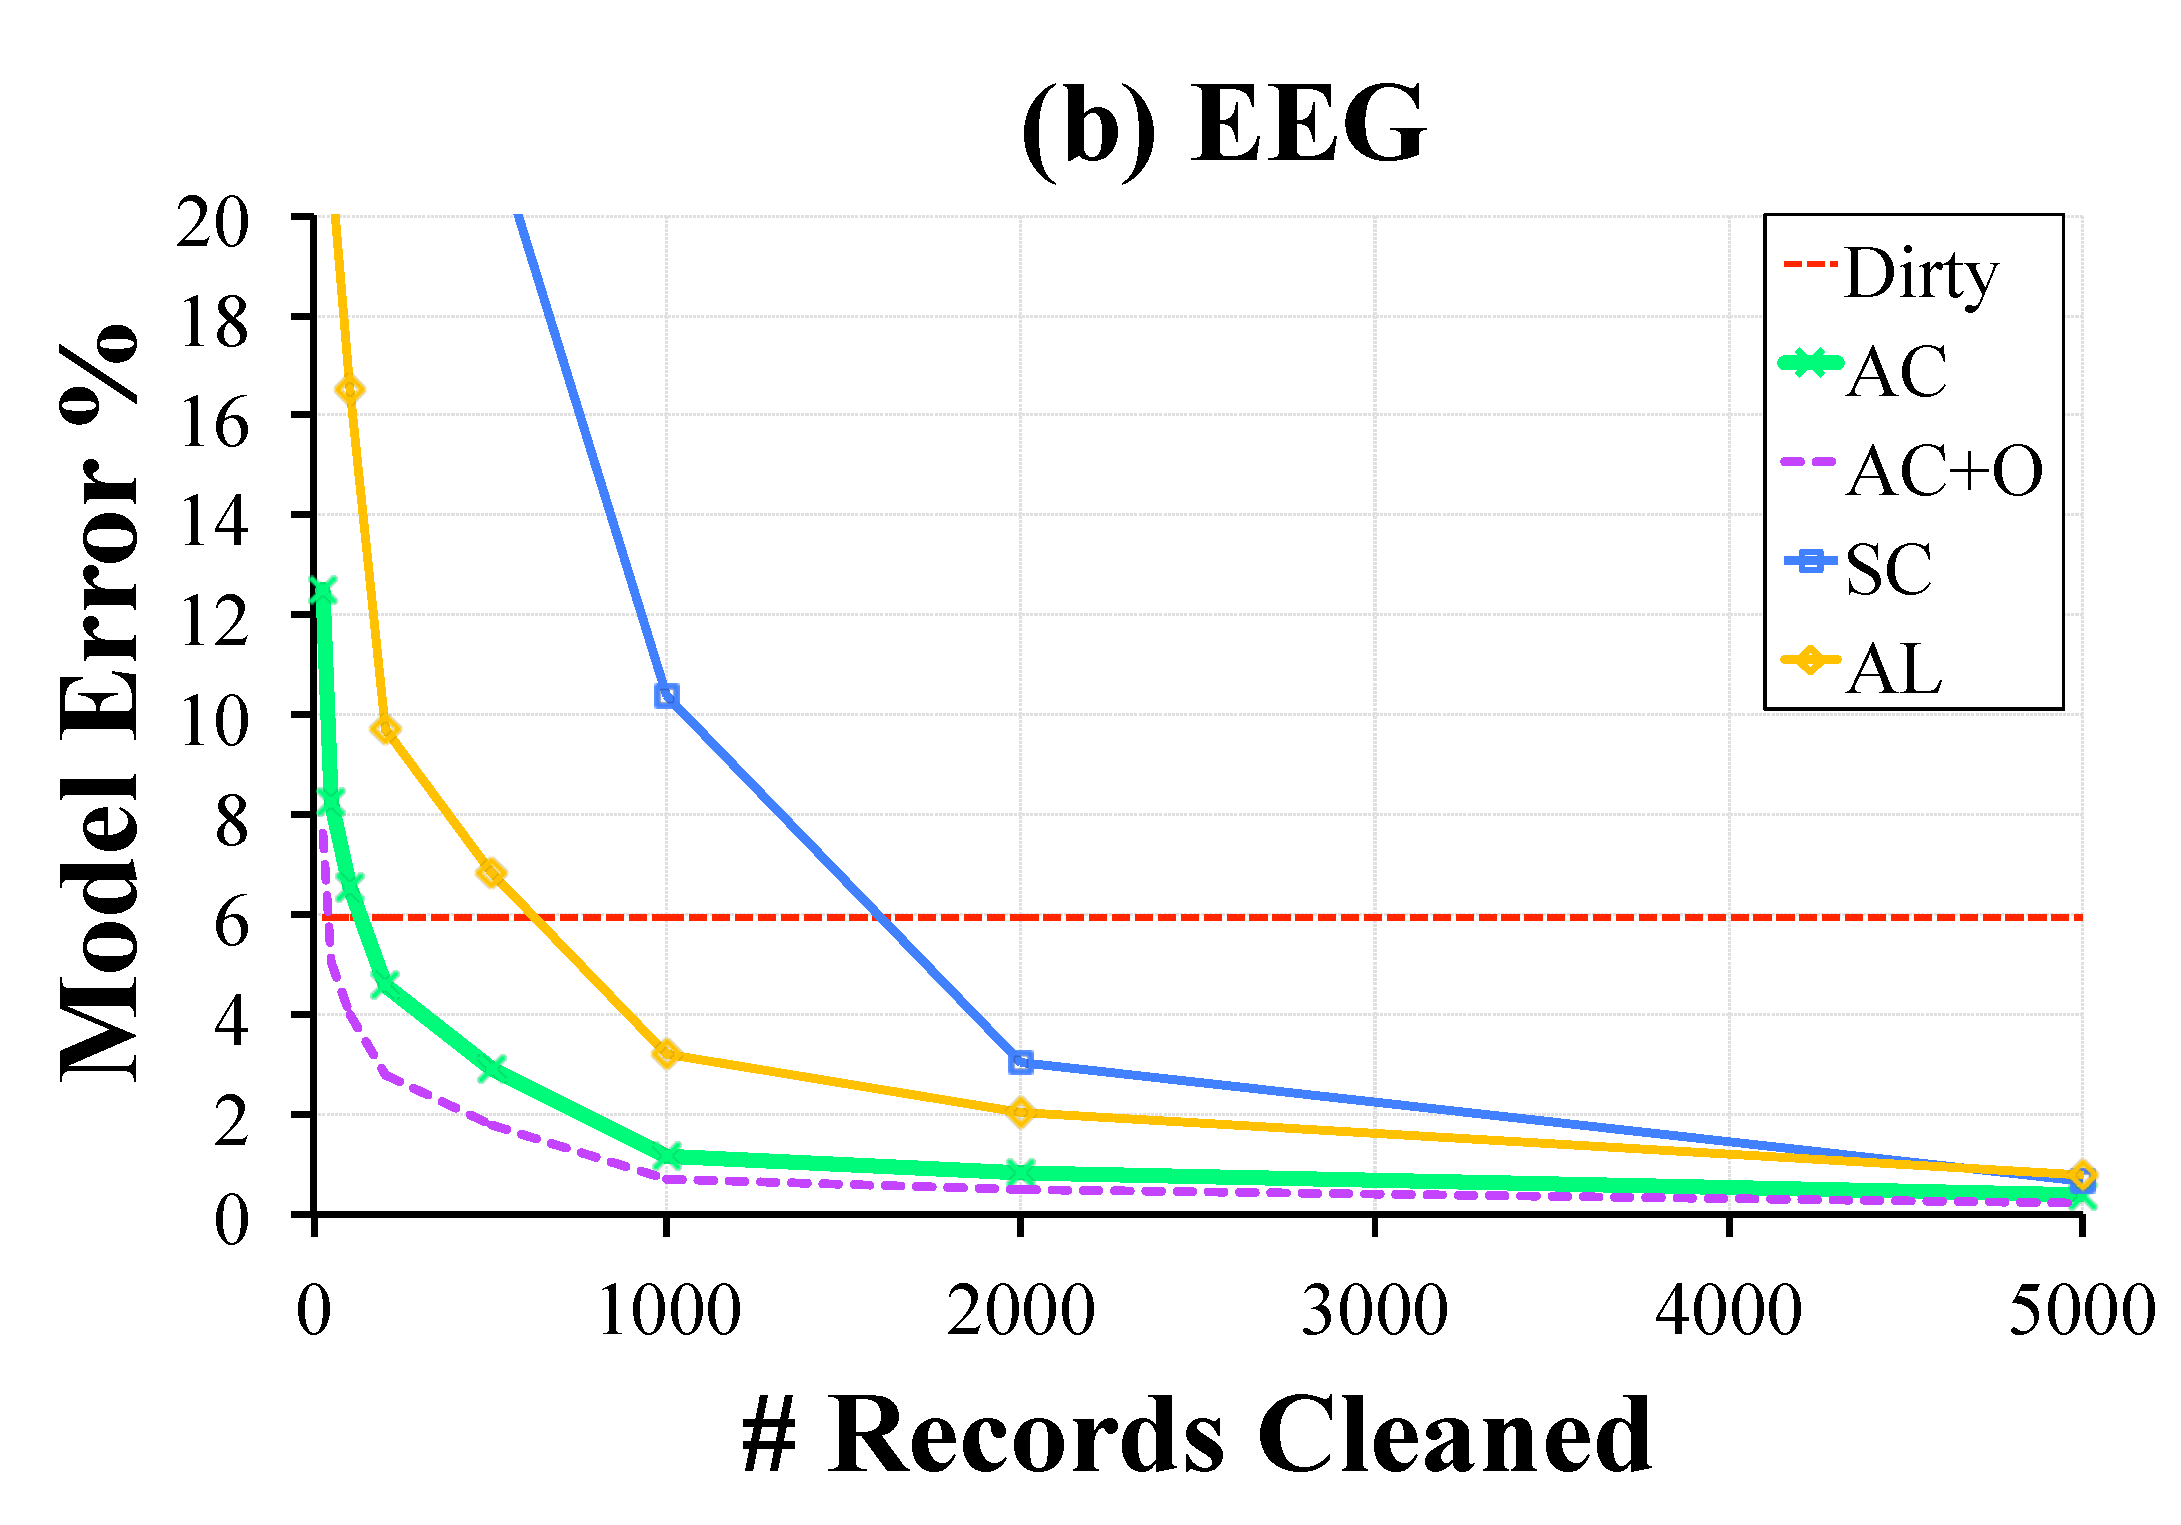
\includegraphics[scale=0.15]{exp/exp3c.pdf}
 \caption{\sys converges with a smaller sample size to the true result in comparison to Active Learning and SampleClean. We show the relative model error (on a log scale) as a function of the number of examples cleaned. \label{prio-perf}}
\end{figure*}

\subsubsection{2b. Source of Improvements}
Throughout the paper, we proposed numerous optimizations.
Now, we try to understand the source of our improvements w.r.t Active Learning and SampleClean.
We pick a single point on the curves shown in Figure \ref{prio-perf} that corresponds to 10\% of the data cleaned (55 for Housing, 4555 for Adult, 150 for EEG) and compare the performance of \sys with and without various optimizations.
We denote \sys without partitioning as (AC-P) and \sys without partitioning and importance sampling as (AC-P-I).
In Figure \ref{opts}, we plot the relative error of the alternatives w.r.t to the optimized version of \sys.
Partitioning significantly improves our results in all of the datasets, and accounts for a substantial part of the improvements over Active Learning.
However, when we remove partitioning we still see some improvements since our importance sampling relies on error impact estimates that judge how valuable a point is to the clean model rather than the dirty model in Active Learning.
Not surprisingly, when we remove both these optimizations, \sys is comparable or slightly worse than Active Learning.

\begin{figure}[ht!]
\centering
 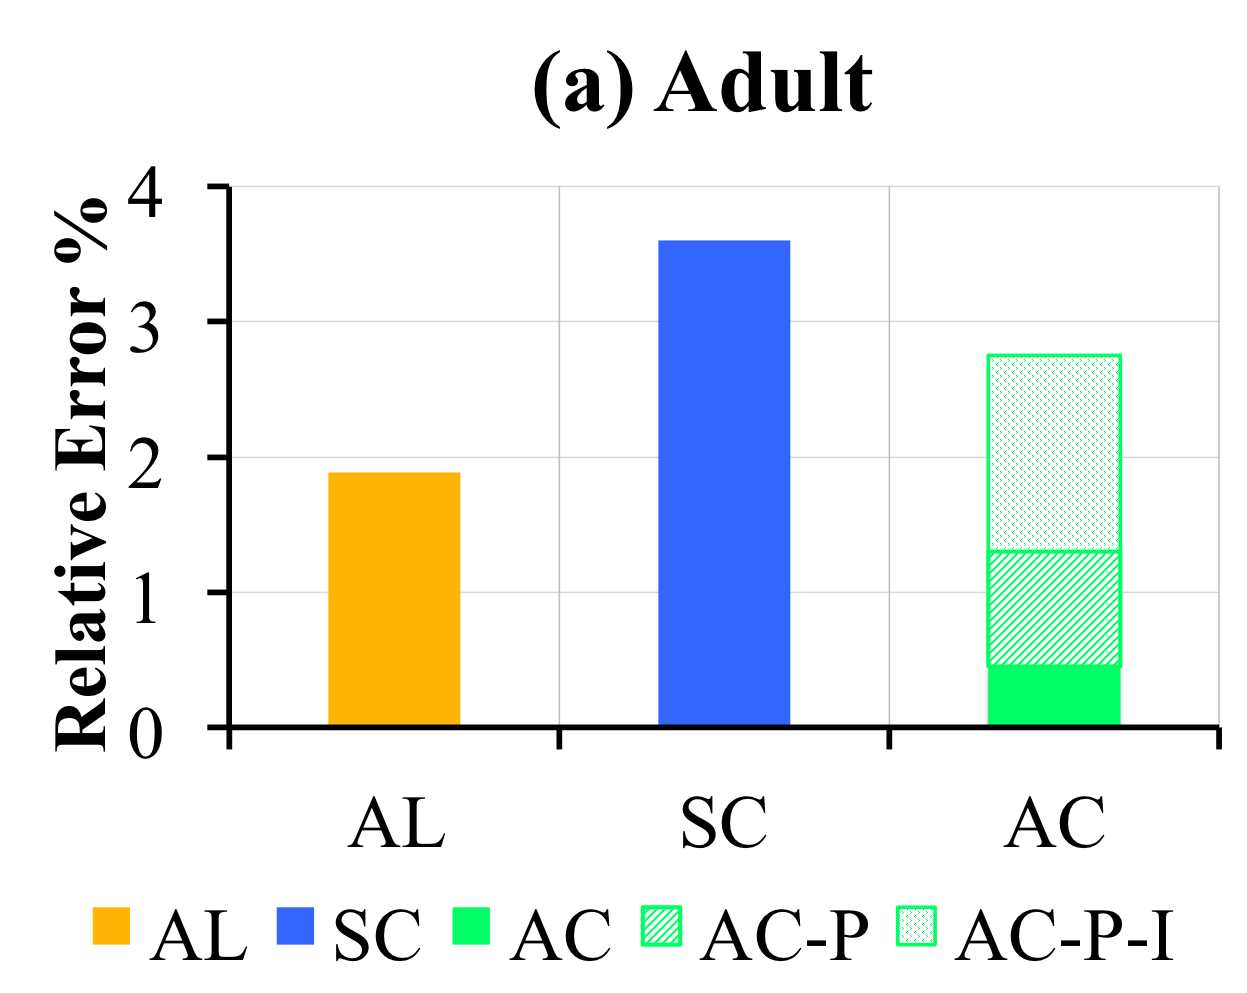
\includegraphics[width=\columnwidth]{exp/exp8.png}
 \caption{We clean 10\% of the data with the alternative algorithms and also include variants of \sys with optimization removed. We plot the relative error w.r.t the optimized \sys. Both partitioning and importance sampling lead to significant reductions in error. \label{opts}}
\end{figure}

We evalue Active Learning and \sys to better understand this relationship.
In Figure \ref{albias}, we vary the biasing effect of our random corruptions.
That is, we start with zero mean noise and increase the mean value and variance of the noise.
Since Active Learning uses the gradient, if there is zero mean noise, in expectation, the dirty data and clean data are the same.
However, as the bias increases, the fact that Active Learning prioritizes w.r.t to the dirty data matters more and becomes increasingly erroneous w.r.t to \sys.

\begin{figure}[ht!]
\centering
 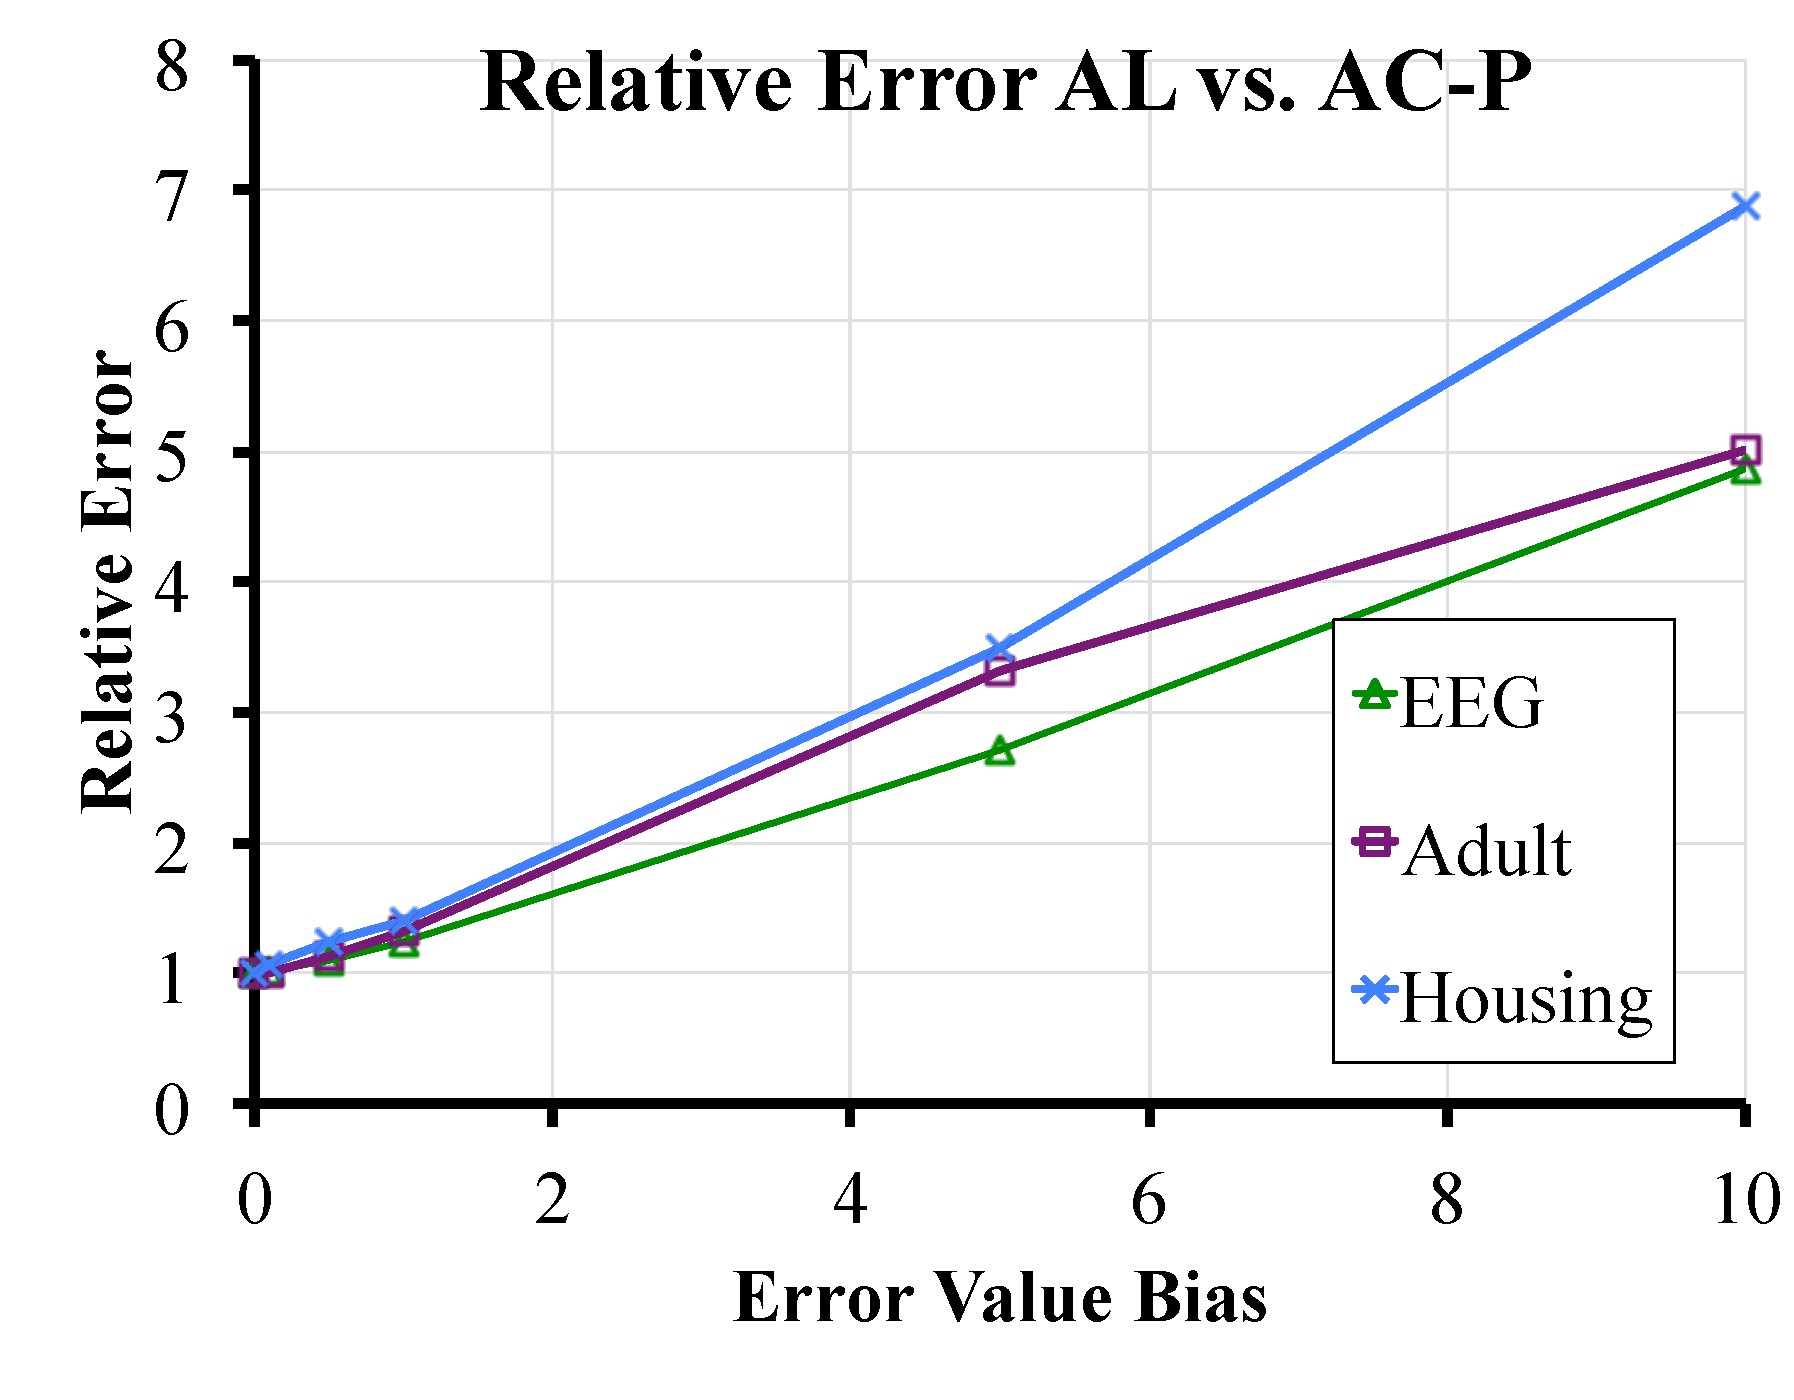
\includegraphics[width=0.6\columnwidth]{exp/exp10.pdf}
 \caption{As we increase the biasing nature of the corruption, Active Learning is increasingly erroneous w.r.t \sys. \label{albias}}
\end{figure}

\subsubsection{2c. Error Dependence}
Both Active Learning and \sys outperform SampleClean in our experiments.
In our next experiment, we try to understand how much of this performance 
is due to the initialization (i.e., SampleClean trains a model from ``scratch").
We vary the rate of random error, thus making the initialization more and more arbitrary, 
and measure the relative performance between SampleClean and \sys.
Since SampleClean only acts on a clean sample of data, it is robust to data error.
So at some point, the errors in the data are so significant that training a model on a small but clean sample of data is more efficient than iteratively updating the dirty model.

In Figure \ref{bias}, we present the results from this experiment.
We corrupt entries from the data matrix of the Adult dataset at random (probability on plotted on the x-axis).
Then, we measure the number of records we need to clean before we have a relative error of 0.1\%.
We find that at about 30\% corruption rate, SampleClean is more accurate than \sys.
Since the Adult dataset has 12 features, a 30\% corruption rate corresponds to each example with 3.6 features incorrect on average.
We optimized \sys for sparse and relatively small errors but it still shows reasonable performance even in this highly erroneous setting. 
At higher corruption rates, \sys requires more than one epoch to converge to an accurate answer which requires cleaning almost all of the data.

\begin{figure}[ht!]
\centering
 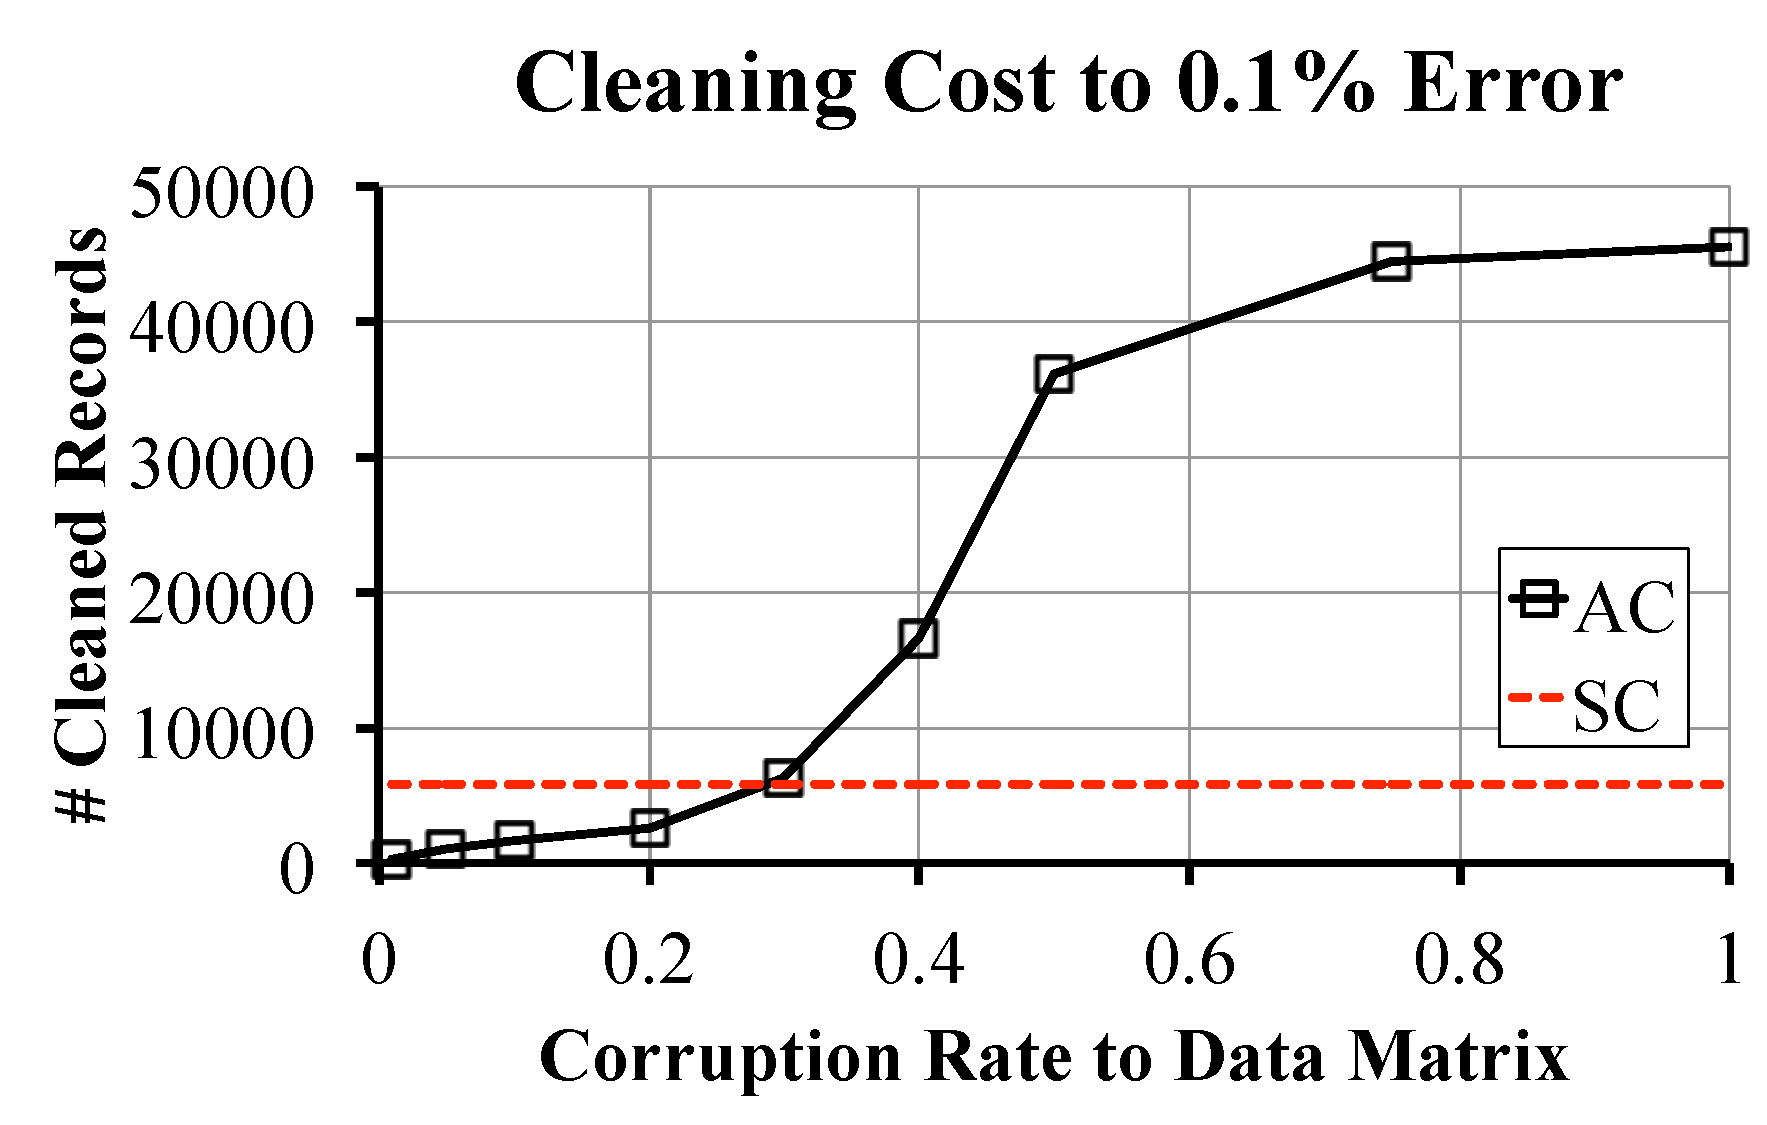
\includegraphics[width=0.6\columnwidth]{exp/exp9.pdf}
 \caption{We corrupt an increasing number of entries in the data matrix. At about 30\% corrupted, \sys is no longer more efficient than SampleClean. \label{bias}}
\end{figure}

\subsubsection{2d. Testing Accuracy}
In the previous experiments, we studied the relative model error which measures the training loss. 
However, to an end user the metric that matters is test accuracy.
In the next experiment, we try to understand how reductions in model error correlate to improvements in test error.
In Figure \ref{prio-tperf}, we present the results for the three datasets: Adult, Housing, and EEG.
We find that in two of the datasets, Housing and Adult, \sys converges to clean test accuracy faster than the alternatives.

However, there is a curious negative result with the EEG dataset that we would like to highlight. 
We find that even though \sys has significantly lower model error (Figure \ref{prio-perf}), this does not correspond to as significant of an increase in test accuracy.
We speculate this is due to the inherrent hardness of the EEG classification problem.
\sys may encourage overfitting at intermediate results for hard classification tasks.
The solution to this problem may be to add additional regularization, thus actually changing the optimization problem.
We hope to explore this problem in further detail in future work.

\begin{figure*}[t]
\centering
 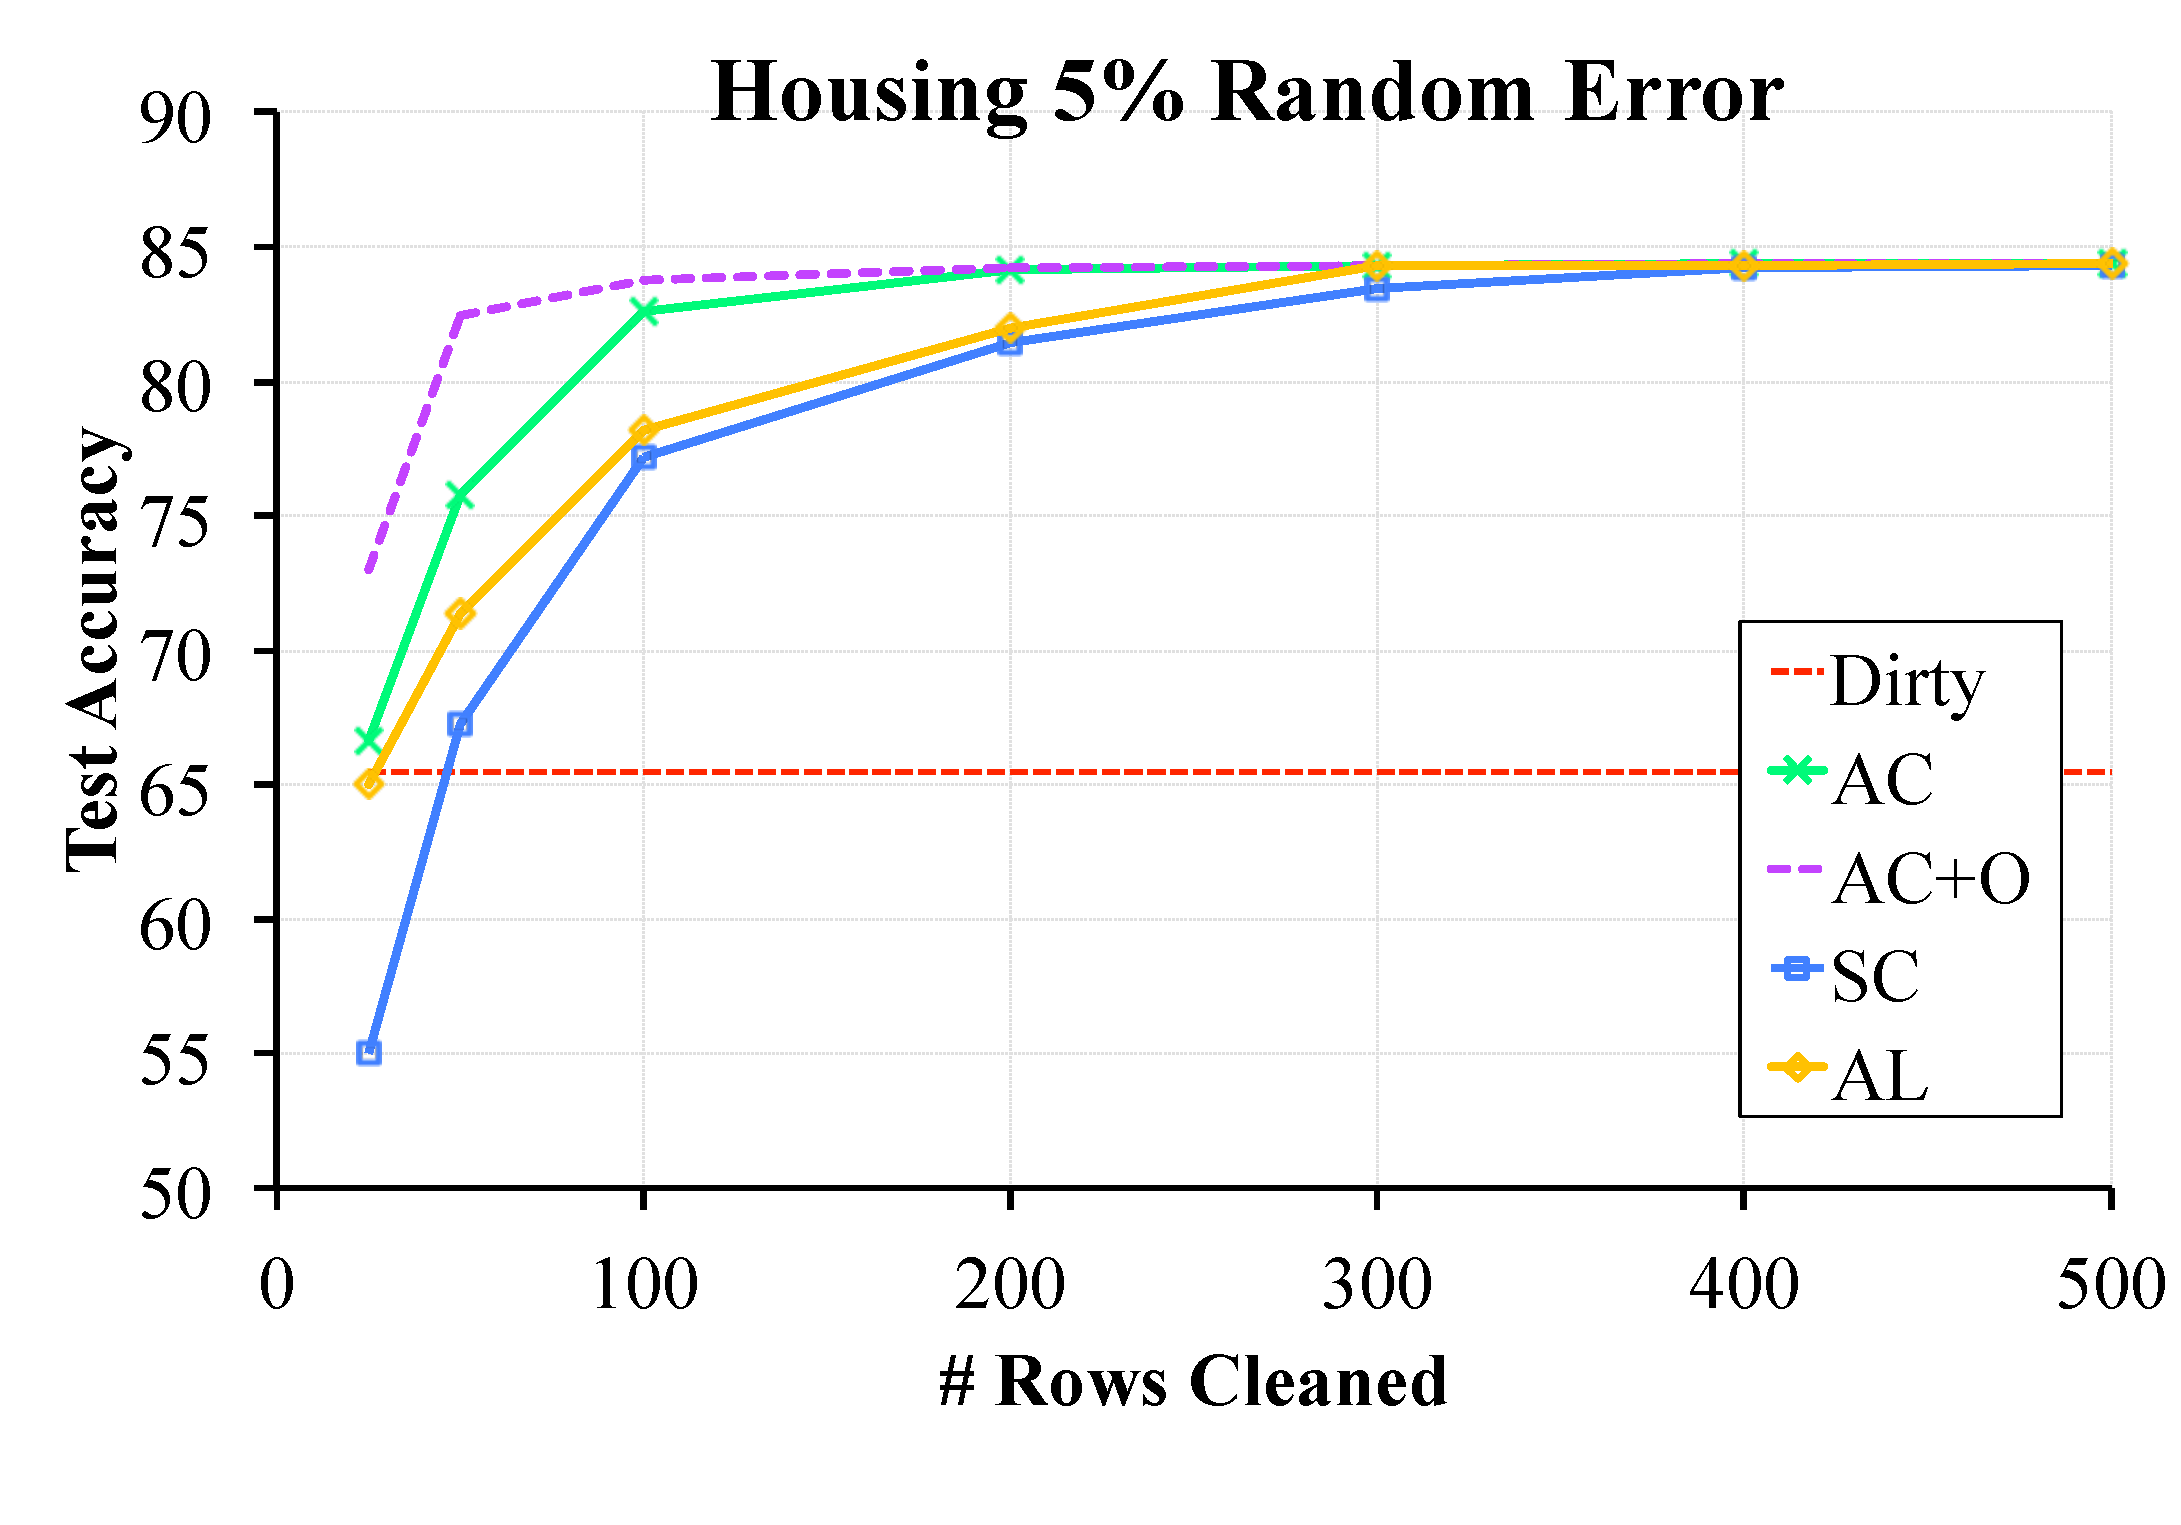
\includegraphics[scale=0.15]{exp/exp3aa.pdf}
 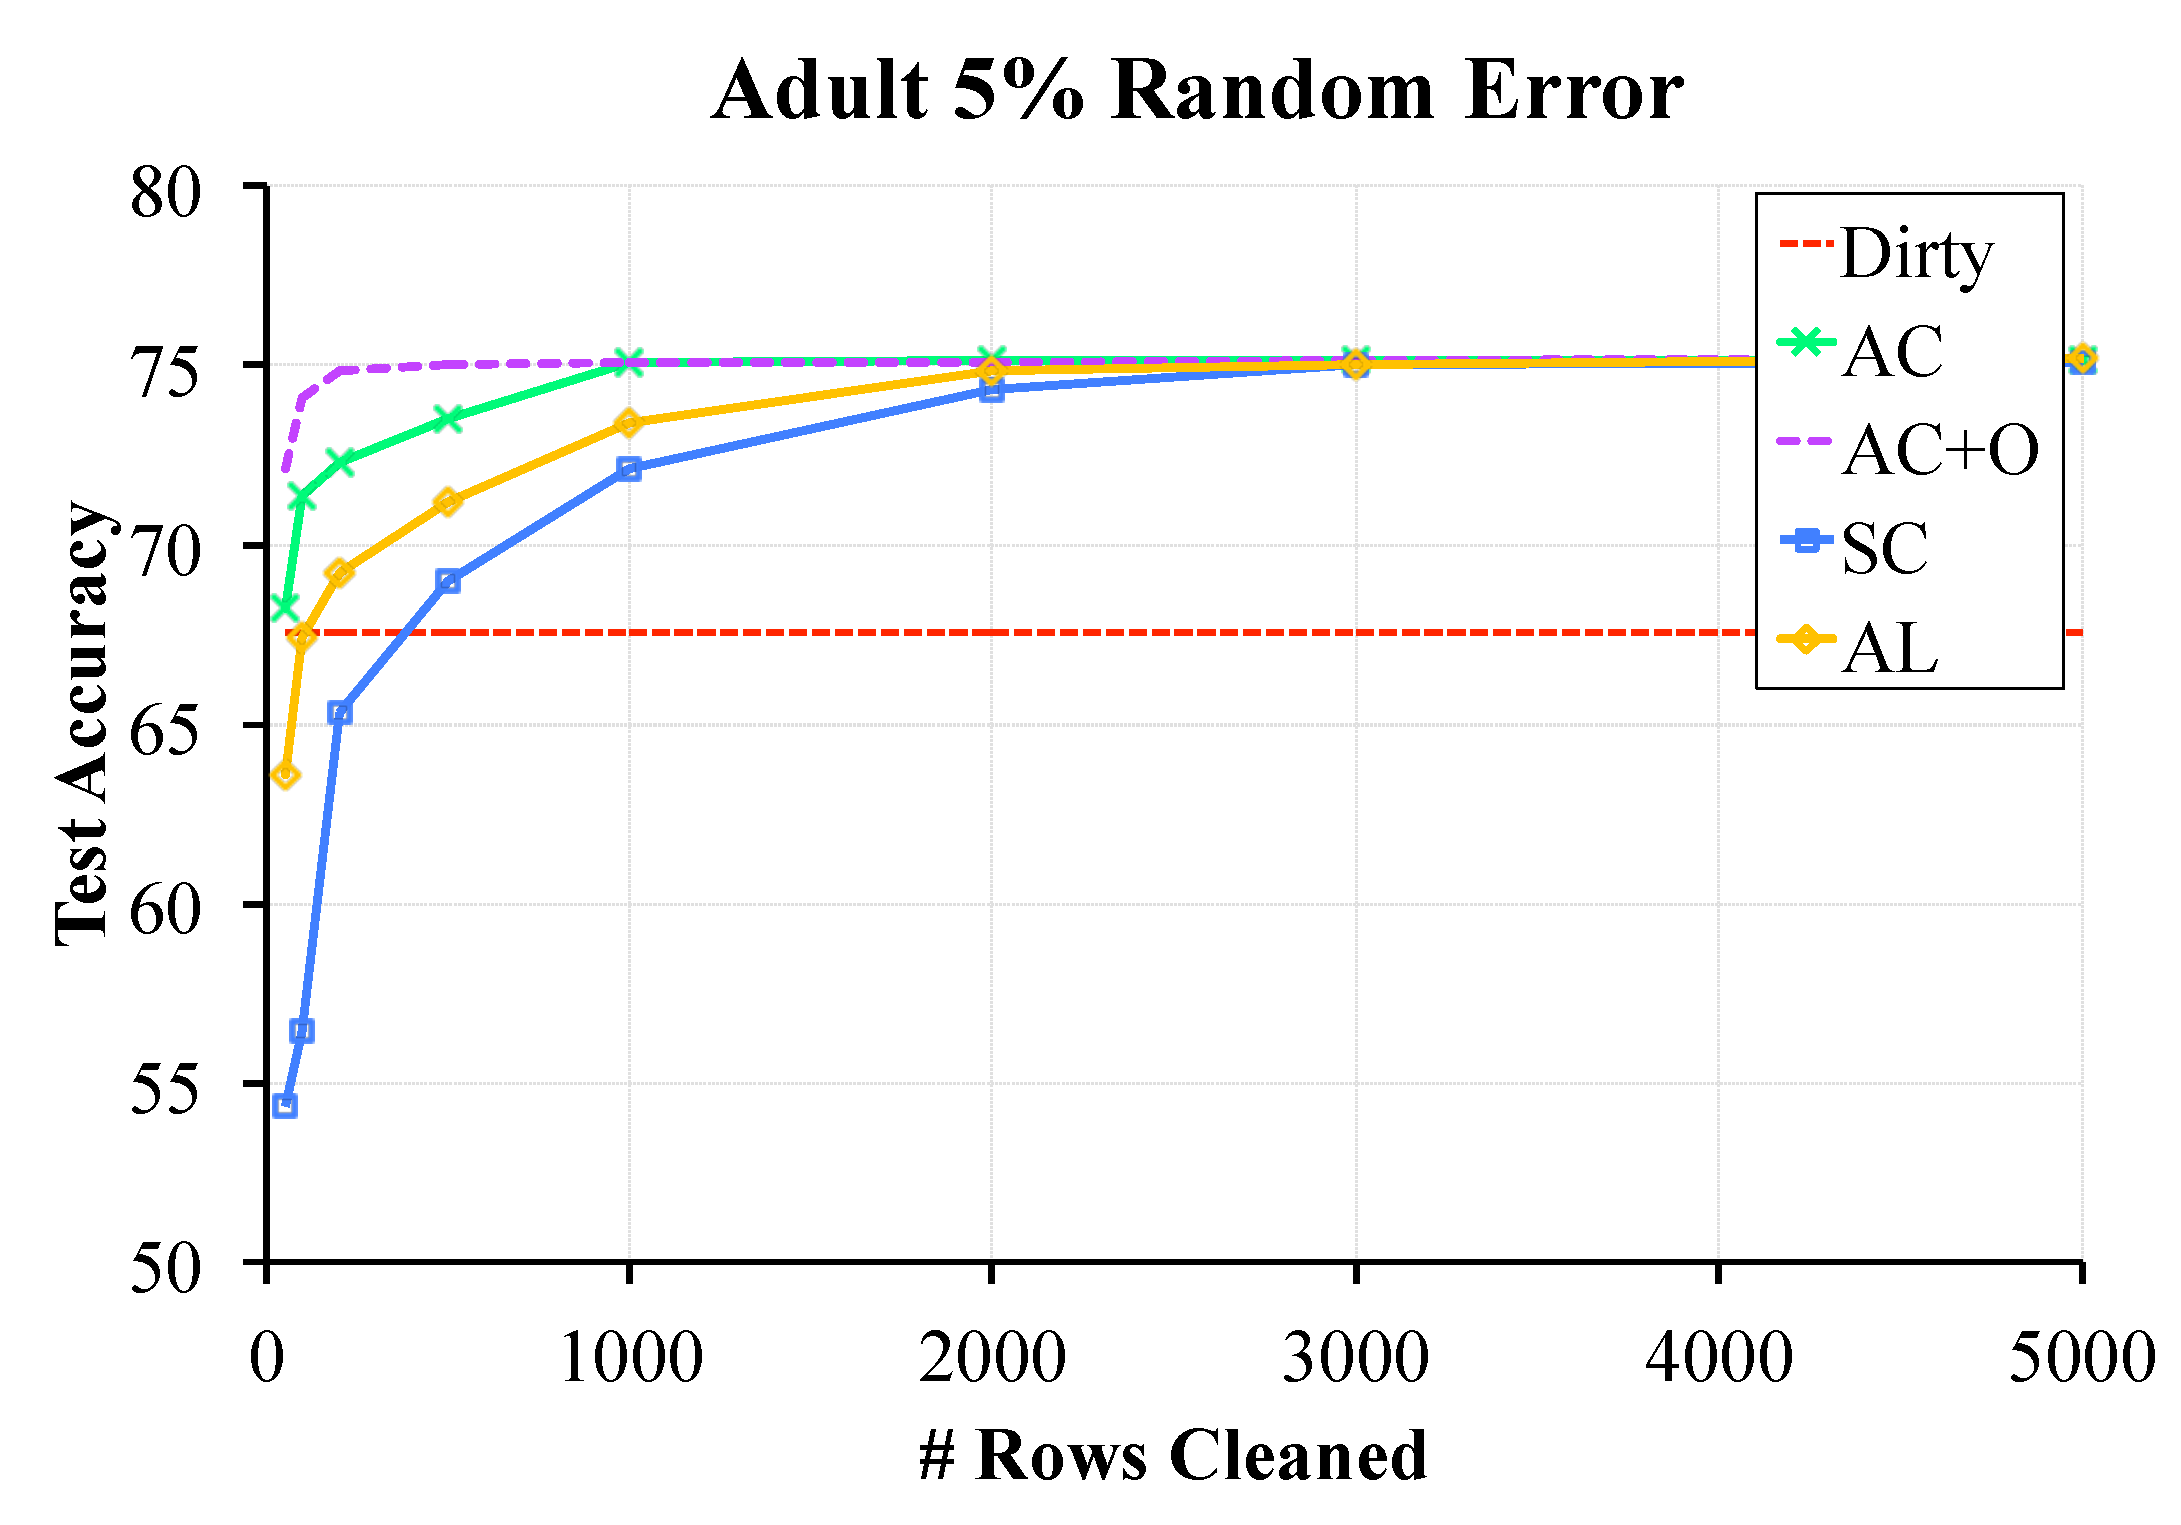
\includegraphics[scale=0.15]{exp/exp3bb.pdf}
  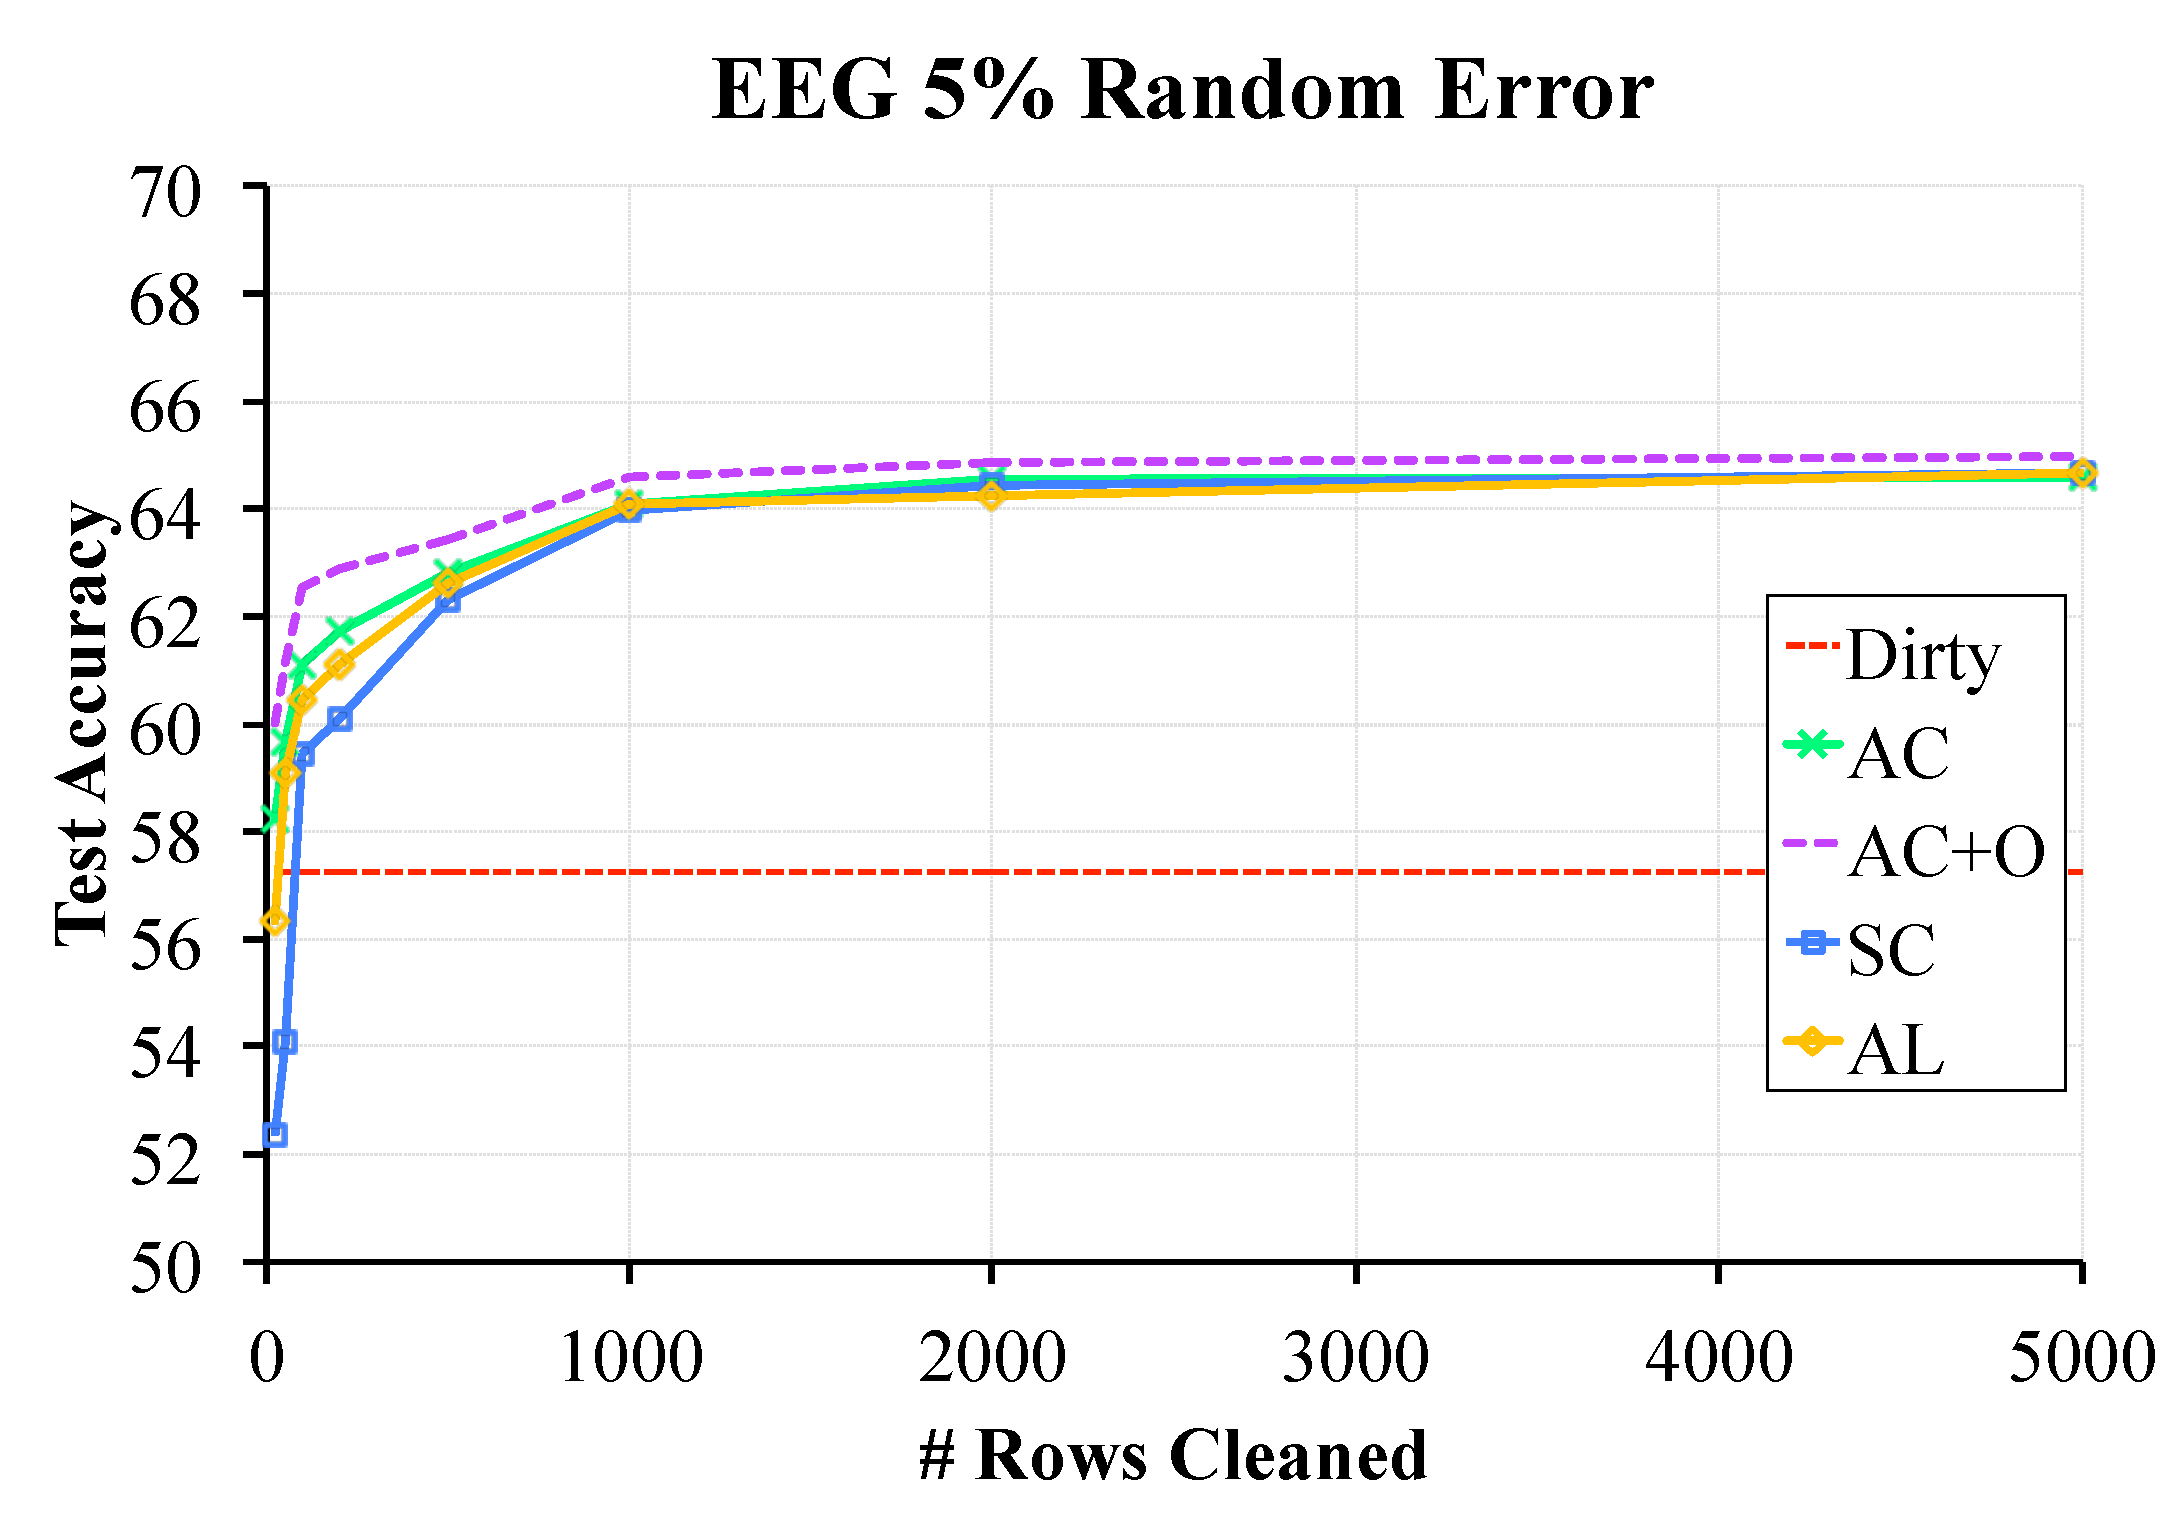
\includegraphics[scale=0.15]{exp/exp3cc.pdf}
 \caption{\sys converges with a smaller sample size to the maximum test accuracy in comparison to Active Learning and SampleClean. The reductions in model error correlate well with increased test accuracy in two of the datasets (a) and (b). In (c), we find insignificant gains in terms of test accuracy. \label{prio-tperf}}
\end{figure*}

\subsection{Experiment 3. Predicates vs. Classification}

\subsubsection{3a. Basic Performance}
In the next set of experiments, we explore the error partitioning in more detail.
We presented two models for error sampling, one where we are given a set of candidate dirty records through a predicate and one where we have to learn this predicate as we clean.
In Figure \ref{pred-perf}, we overlay the convergence plots in the previous experiments with a curve (denoted by AC+C) that represents \sys using a classifier instead of an error predicate.
We use an SVM classifier to predict errors.
We find an interesting tradeoff where initially \sys is comparable to Active Learning (explanation for why seen in Figure \ref{opts}), as our classifier becomes more effective the partitioning improves the performance.

\begin{figure}[t]
\centering
 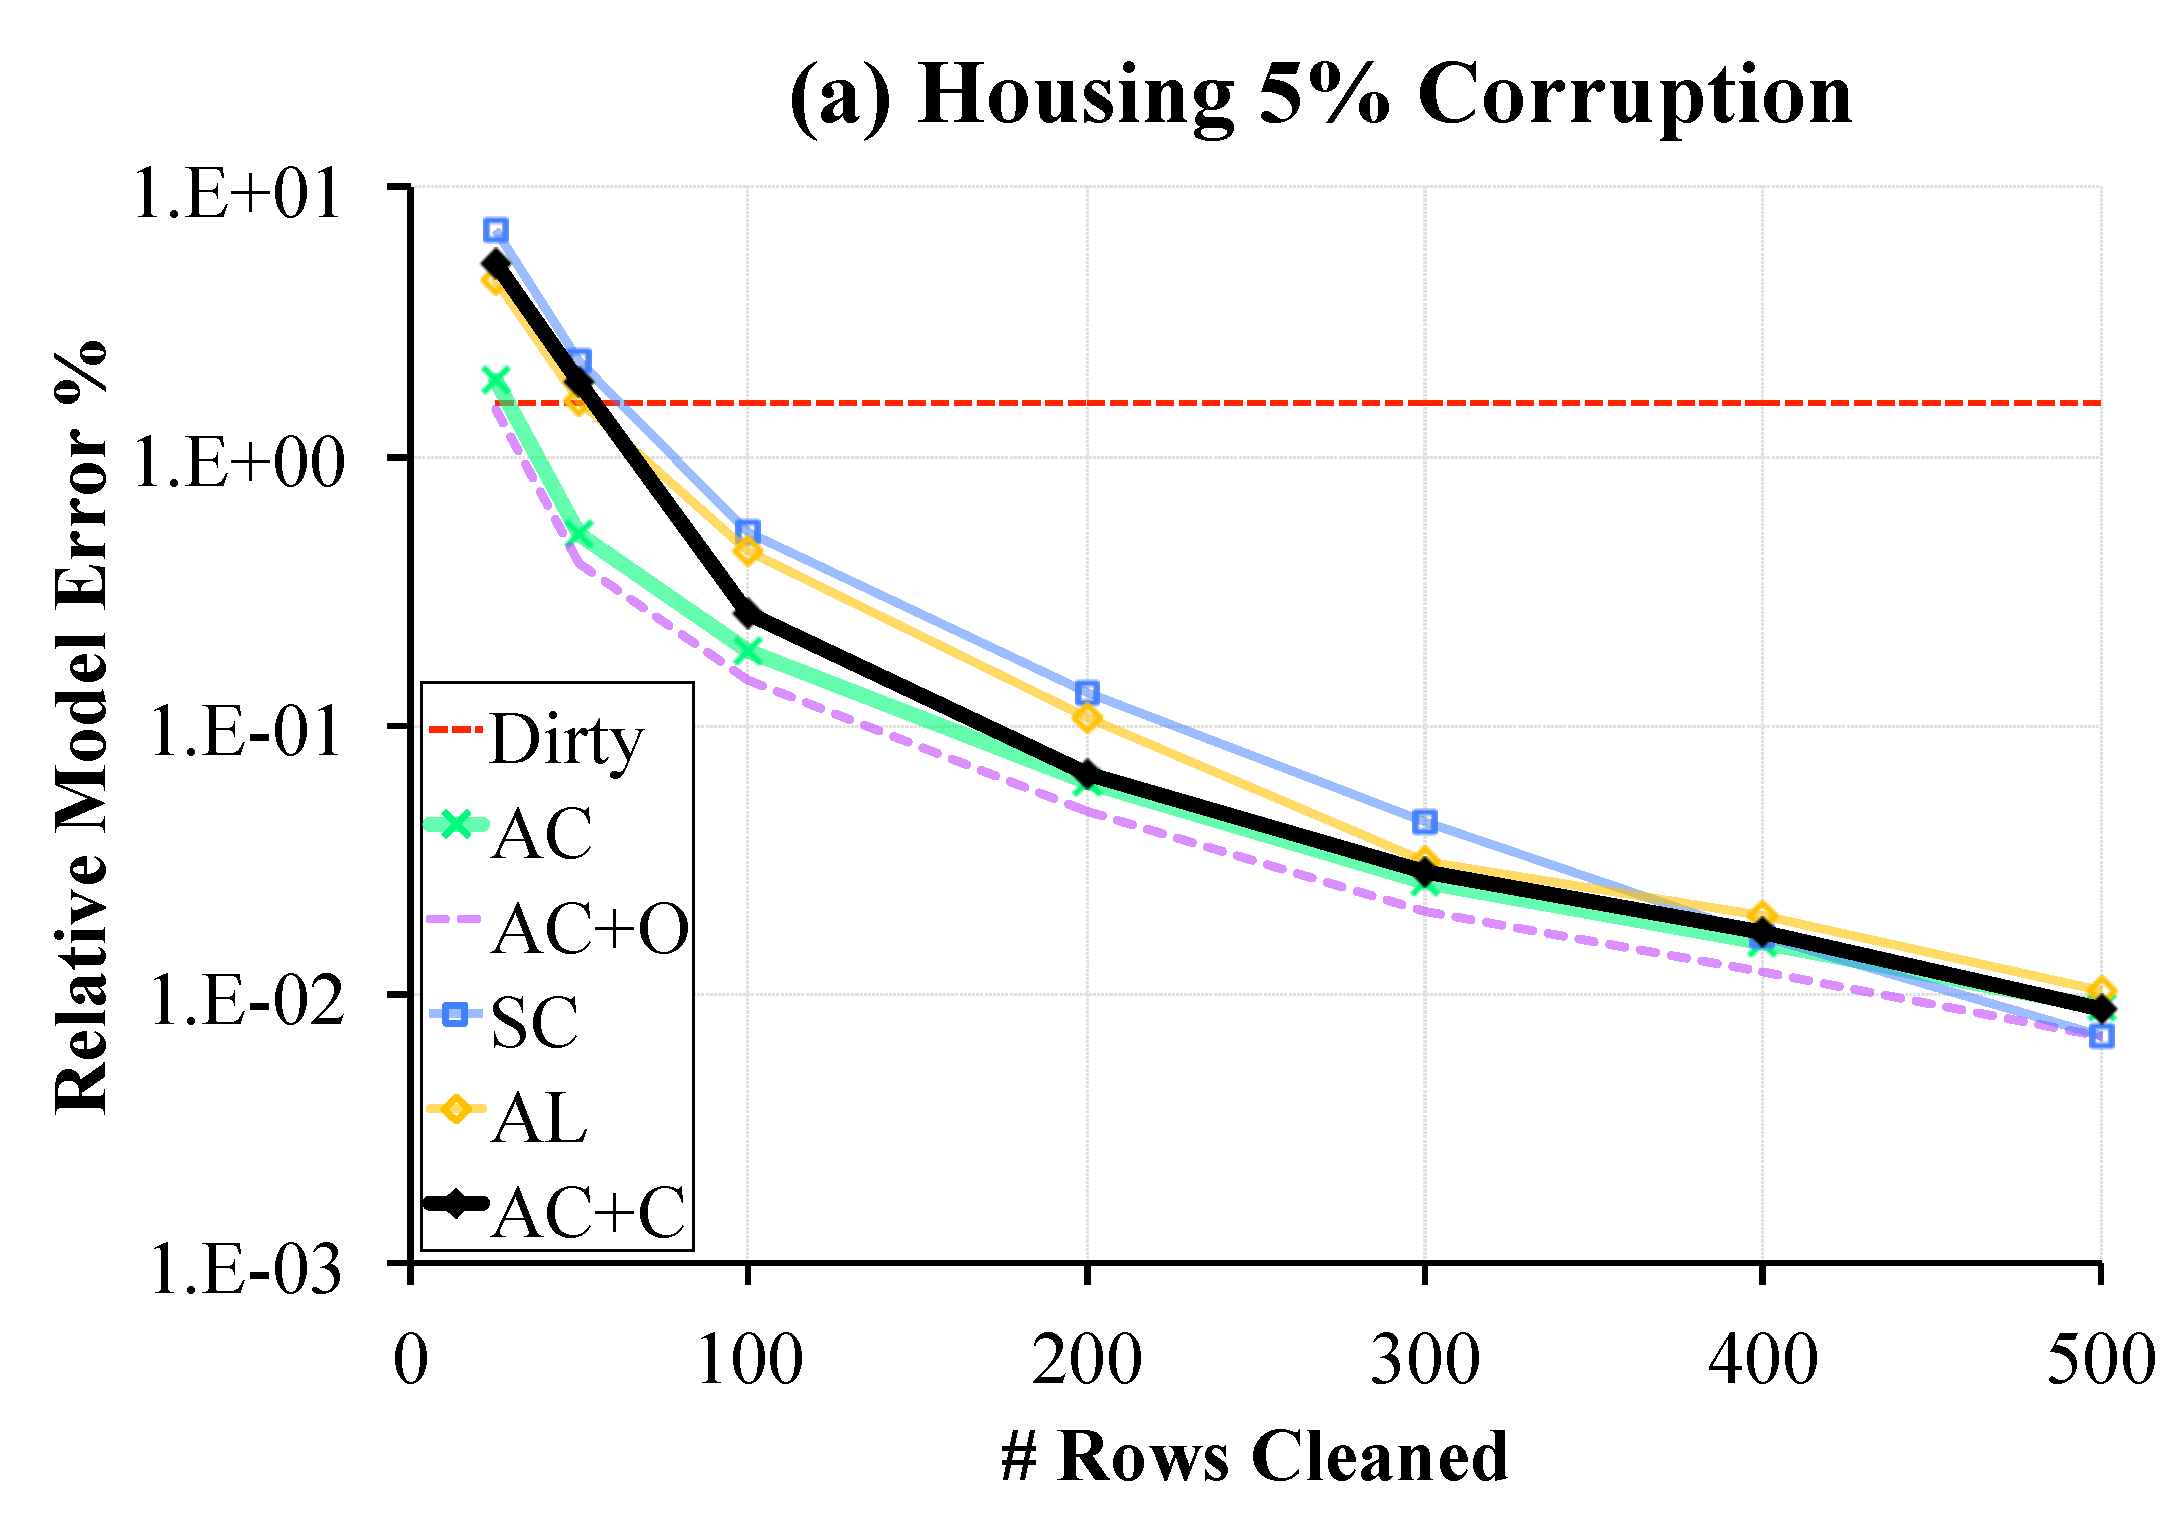
\includegraphics[width=0.48\columnwidth]{exp/exp11a.pdf}
 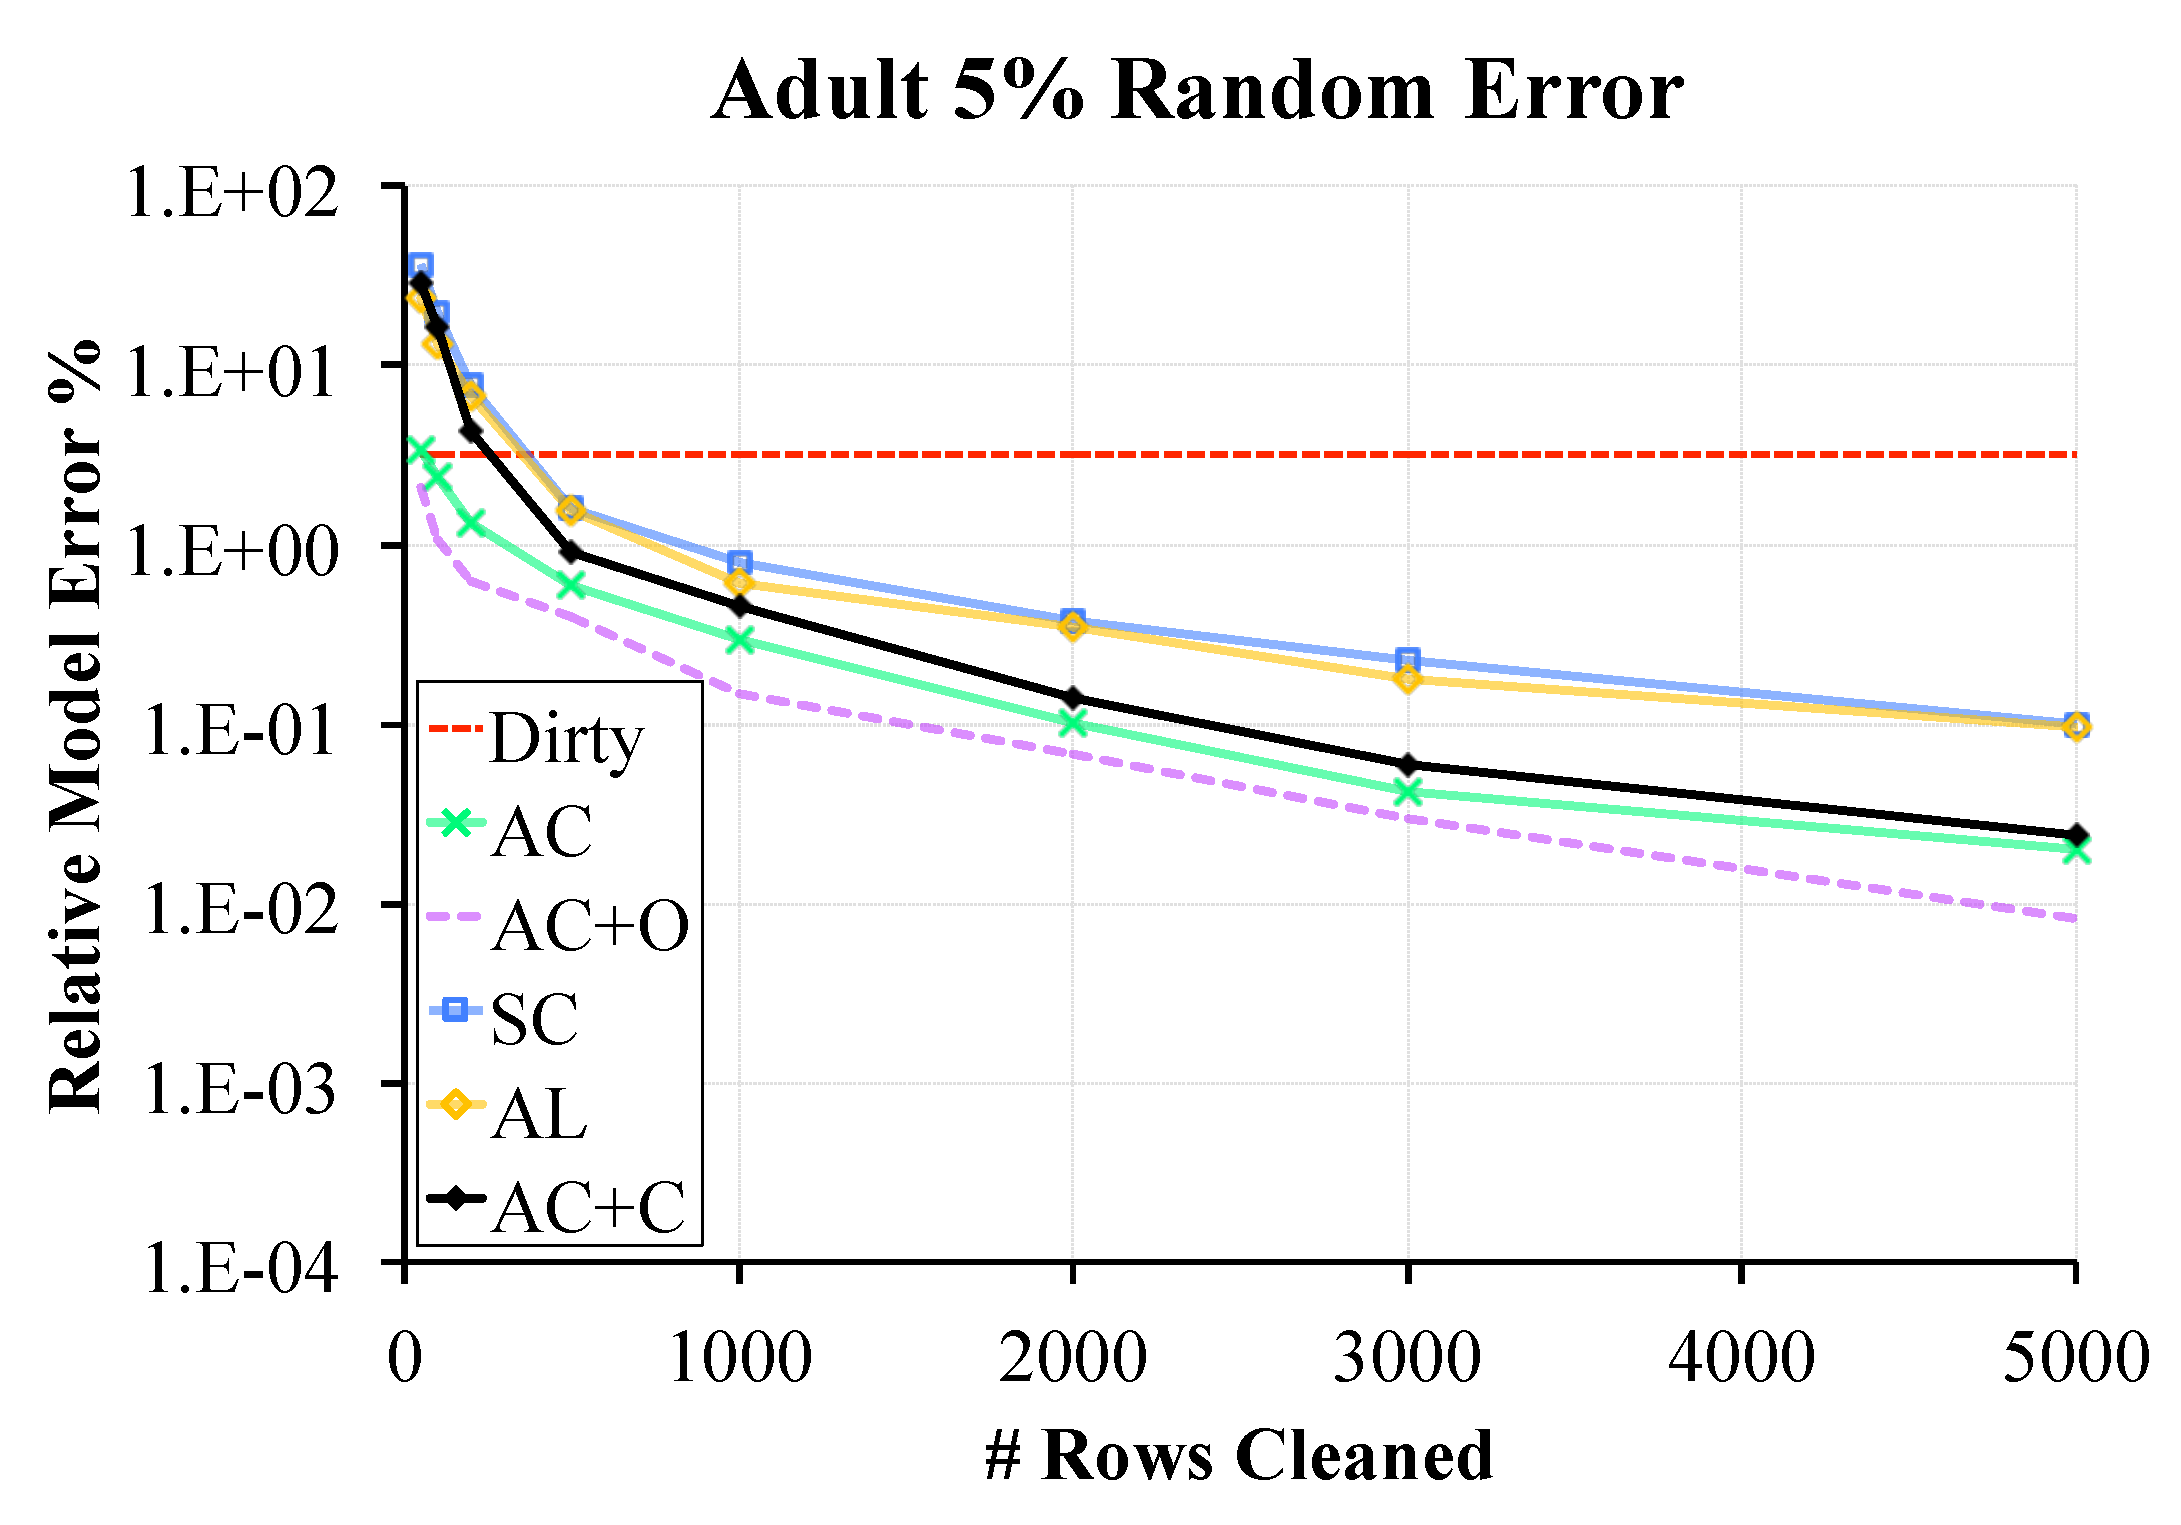
\includegraphics[width=0.48\columnwidth]{exp/exp11b.pdf}
 \caption{Even with a classifier \sys converges faster than Active Learning and SampleClean.
 We plot the error on a log scale. 
 However, initially \sys is comparable in performance to Active Learning, as the classifier acquires training data. \label{pred-perf}}
\end{figure}

\subsubsection{3b. Classifiable Errors}
Using a classifier to partition errors depends on errors that can be classified.
For example, random errors that look like other data may be hard to learn.
As errors become more random, the classifier becomes increasingly erroneous.
We run an experiment where we start with the systematic errors described earlier.
With probability $p$, we increasingly make these errors more random.
We compare these results to AC-P where we do not partition the errors.
In Figure \ref{tradeoffs2}, we plot the error reduction using a classifier.
We find that when errors are about 40\% random then we reach a break even point
where the user is better of not partitiong the data since the errors introduced by incorrect classification are more than the error reductions.

\begin{figure}[ht!]
\centering
 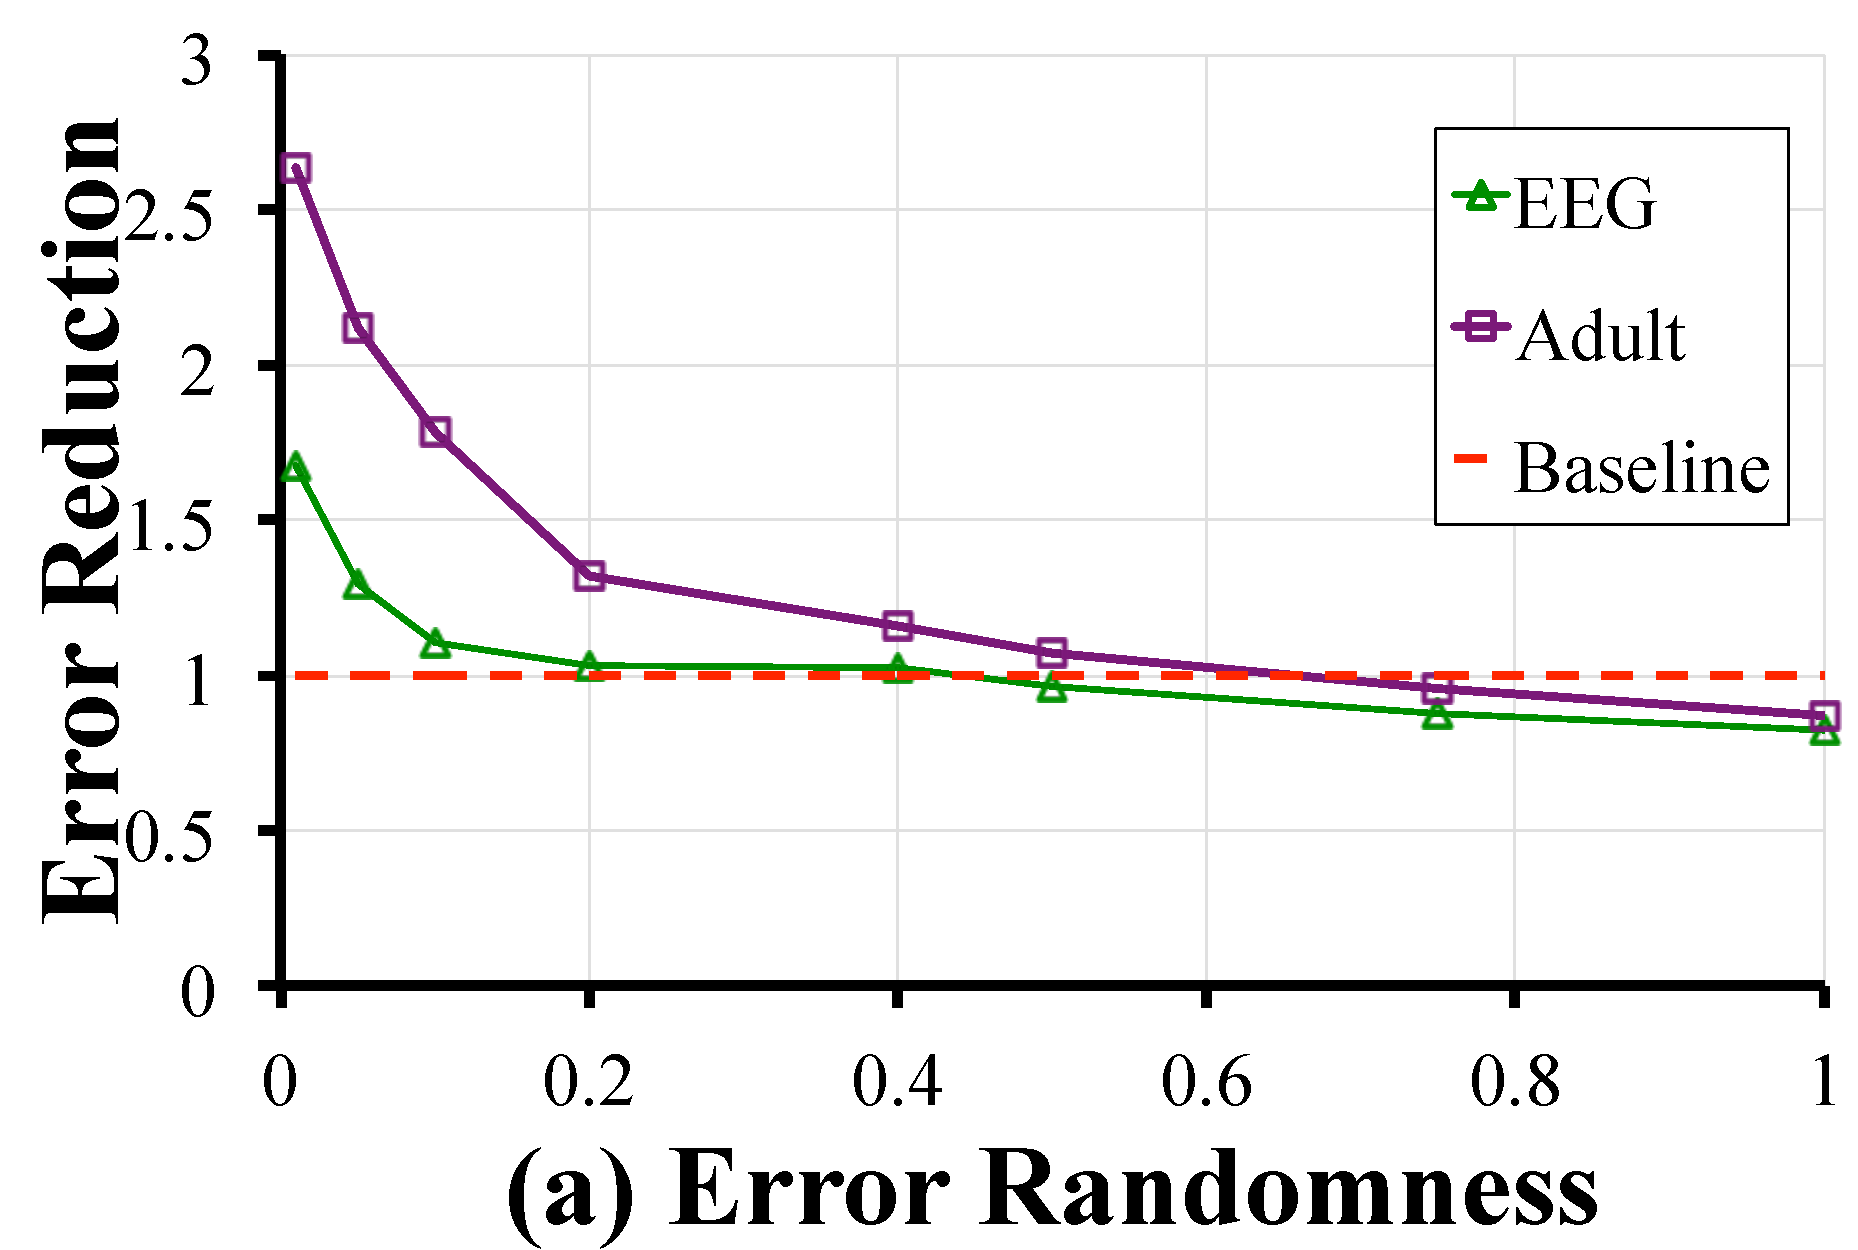
\includegraphics[scale=0.13]{exp/exp5a.pdf}
 \caption{Errors that are less random are easier to classify, and lead to more significant reductions in relative model error. \label{tradeoffs2}}
\end{figure}

\subsection{Experiment 4. Price of a Scan}
In our fourth set of experiments, we evaluate one of the computational premises of our work.
We argue that the price of a scan of data is cheap compared to data cleaning.
The overheads of partioning the dirty and clean data and calculating the sampling distribution should be small in comparison to the faster convergence of our model.
\reminder{How do we quantify the costs of data cleaning?} 

\subsection{Real Scenarios}
We evaluate \sys in two real scenarios: base data replacement and constraint-based data repair.

\subsubsection{Replacing Corrupted Data}
We consider the following scenario with the MNIST handwritten digit recognition dataset.
Suppose, our goal is to classify digits into a set of classes.
However, we suspect that some of our raw images are of low quality.
Typicaly image processing workflows are long with many different featurization steps.
As a result, changes to the raw images may have very significant effects on some features.
In this scenario, the analyst must inspect a potentially corrupted image and replace it with a higher quality one.

The MNIST dataset consists of 64x64 grayscale images.
We run two experiments, in which we have two types of corruptions: (1) 5x5 block removal where take a random 5x5 block from the image and set its pixel values to 0, and (2) Fuzzy where we run a 4x4 moving average over the entire image.
We applied these corruptions to a random 5\% of the images.
In Figure \ref{mnist-corr}, we visualize the corruptions.
We constructed these features to mimic the random vs. systematic errors that we studied before.
The 5x5 block removal behaves much more like a systematic error. 
Typical image processing features are based on edges and corrupting edges leads to ambiguities (e.g., is the image in Figure \ref{mnist-corr} a 4 or a 9).
On the other hand, the making the image fuzzy is more like a random error.

\begin{figure}[ht]
\centering
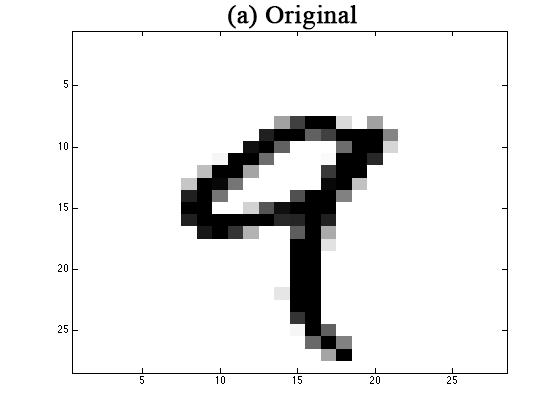
\includegraphics[scale=0.20]{exp/original.png}
 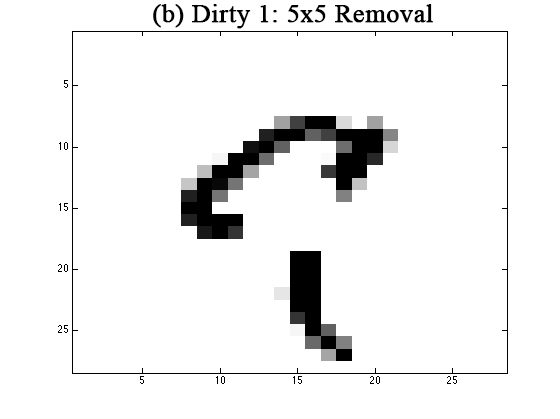
\includegraphics[scale=0.20]{exp/5x5removal.png}
 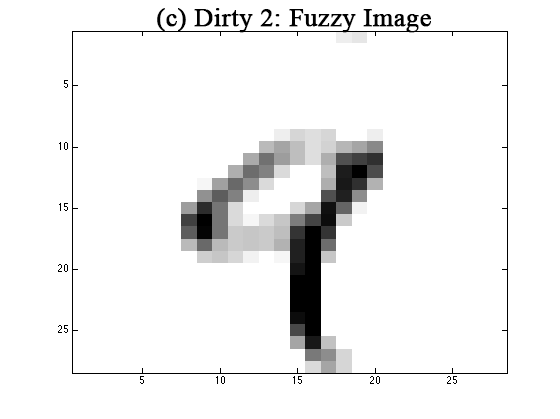
\includegraphics[scale=0.20]{exp/fuzzy.png}
 \caption{We experiment with two forms of corruption in the MNIST image datasets: 5x5 block removal and making the images fuzzy. Image (a) shows an uncorrupted ``9", image (b) shows one corrupted with block removal, and image (c) shows one that is corrupted with fuzziness. \label{mnist-corr}}
\end{figure}

In Figure \ref{mnist}, we present the results.
As in our earlier experiments, we find that \sys makes more progress towards the clean model with a smaller number of examples cleaned.
This experiment highlights a few other interesting points.
First, SampleClean converges at the same rate independent of the data error.
This is because SampleClean does not depend on any quantity derived from the dirty data.
Next, the gap between the theoretical AC+O and what we are able to achieve is much larger in this dataset.
We speculate that this is because classifying errors in a 784 dimensional space is much harder than in our previous experiments, and this in turn leads to reduced accuracy in impact estimation.


\begin{figure}[ht]
\centering
 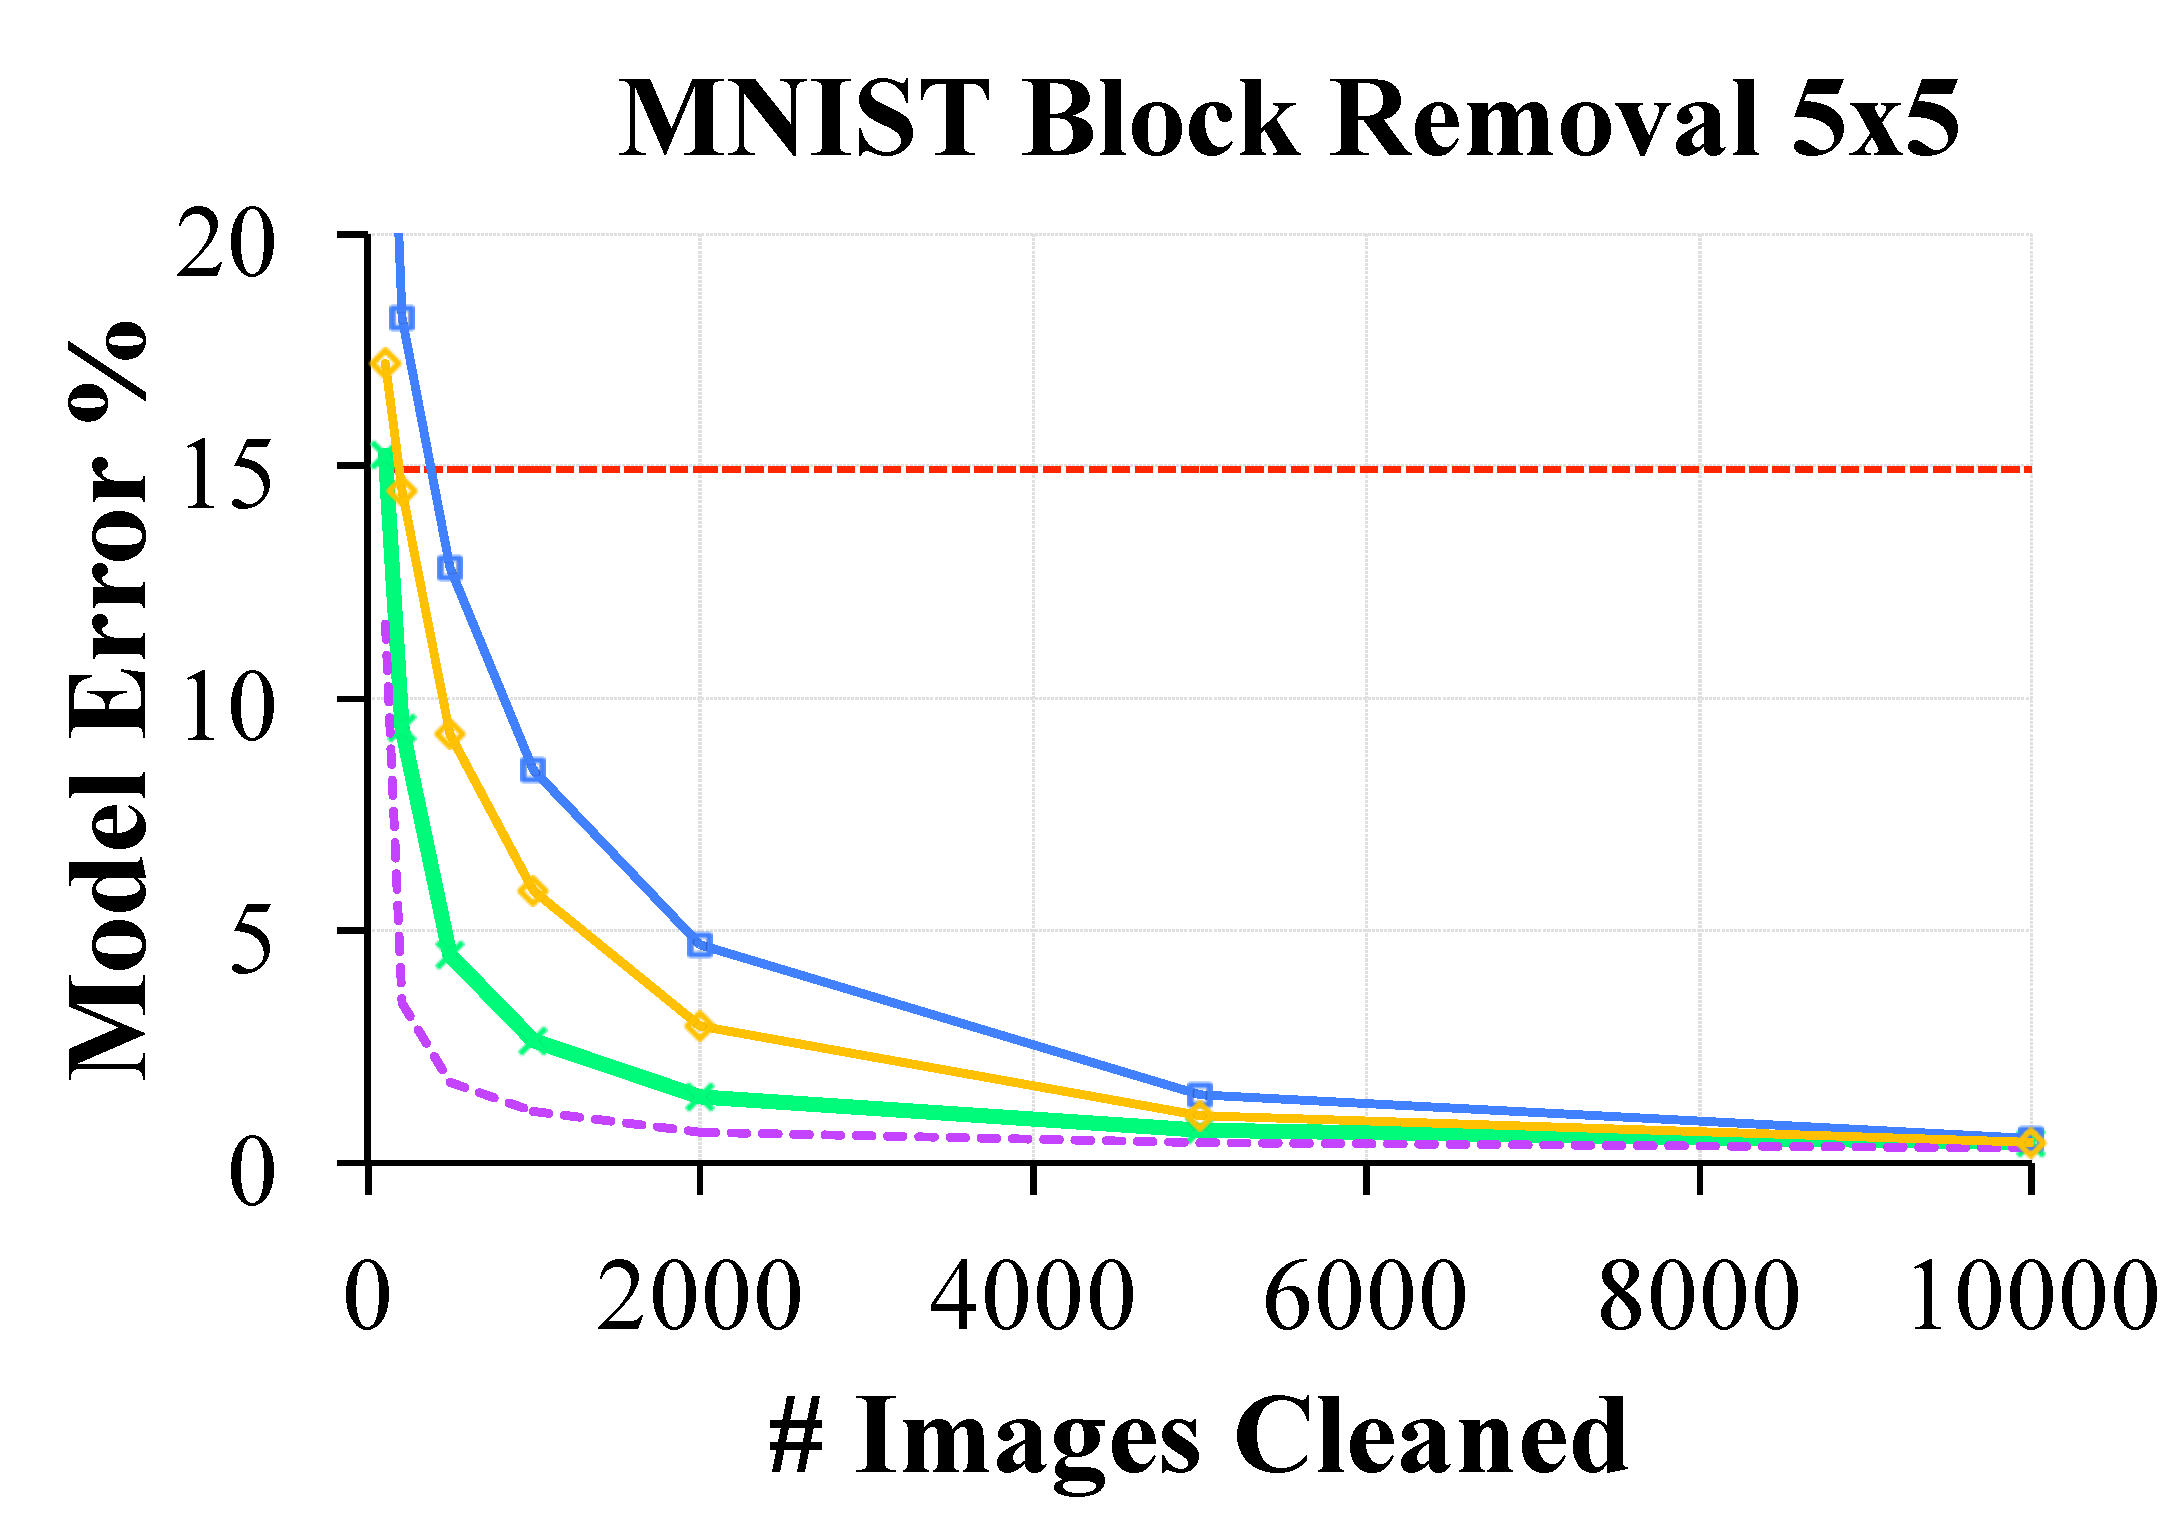
\includegraphics[scale=0.16]{exp/exp7a.pdf}
 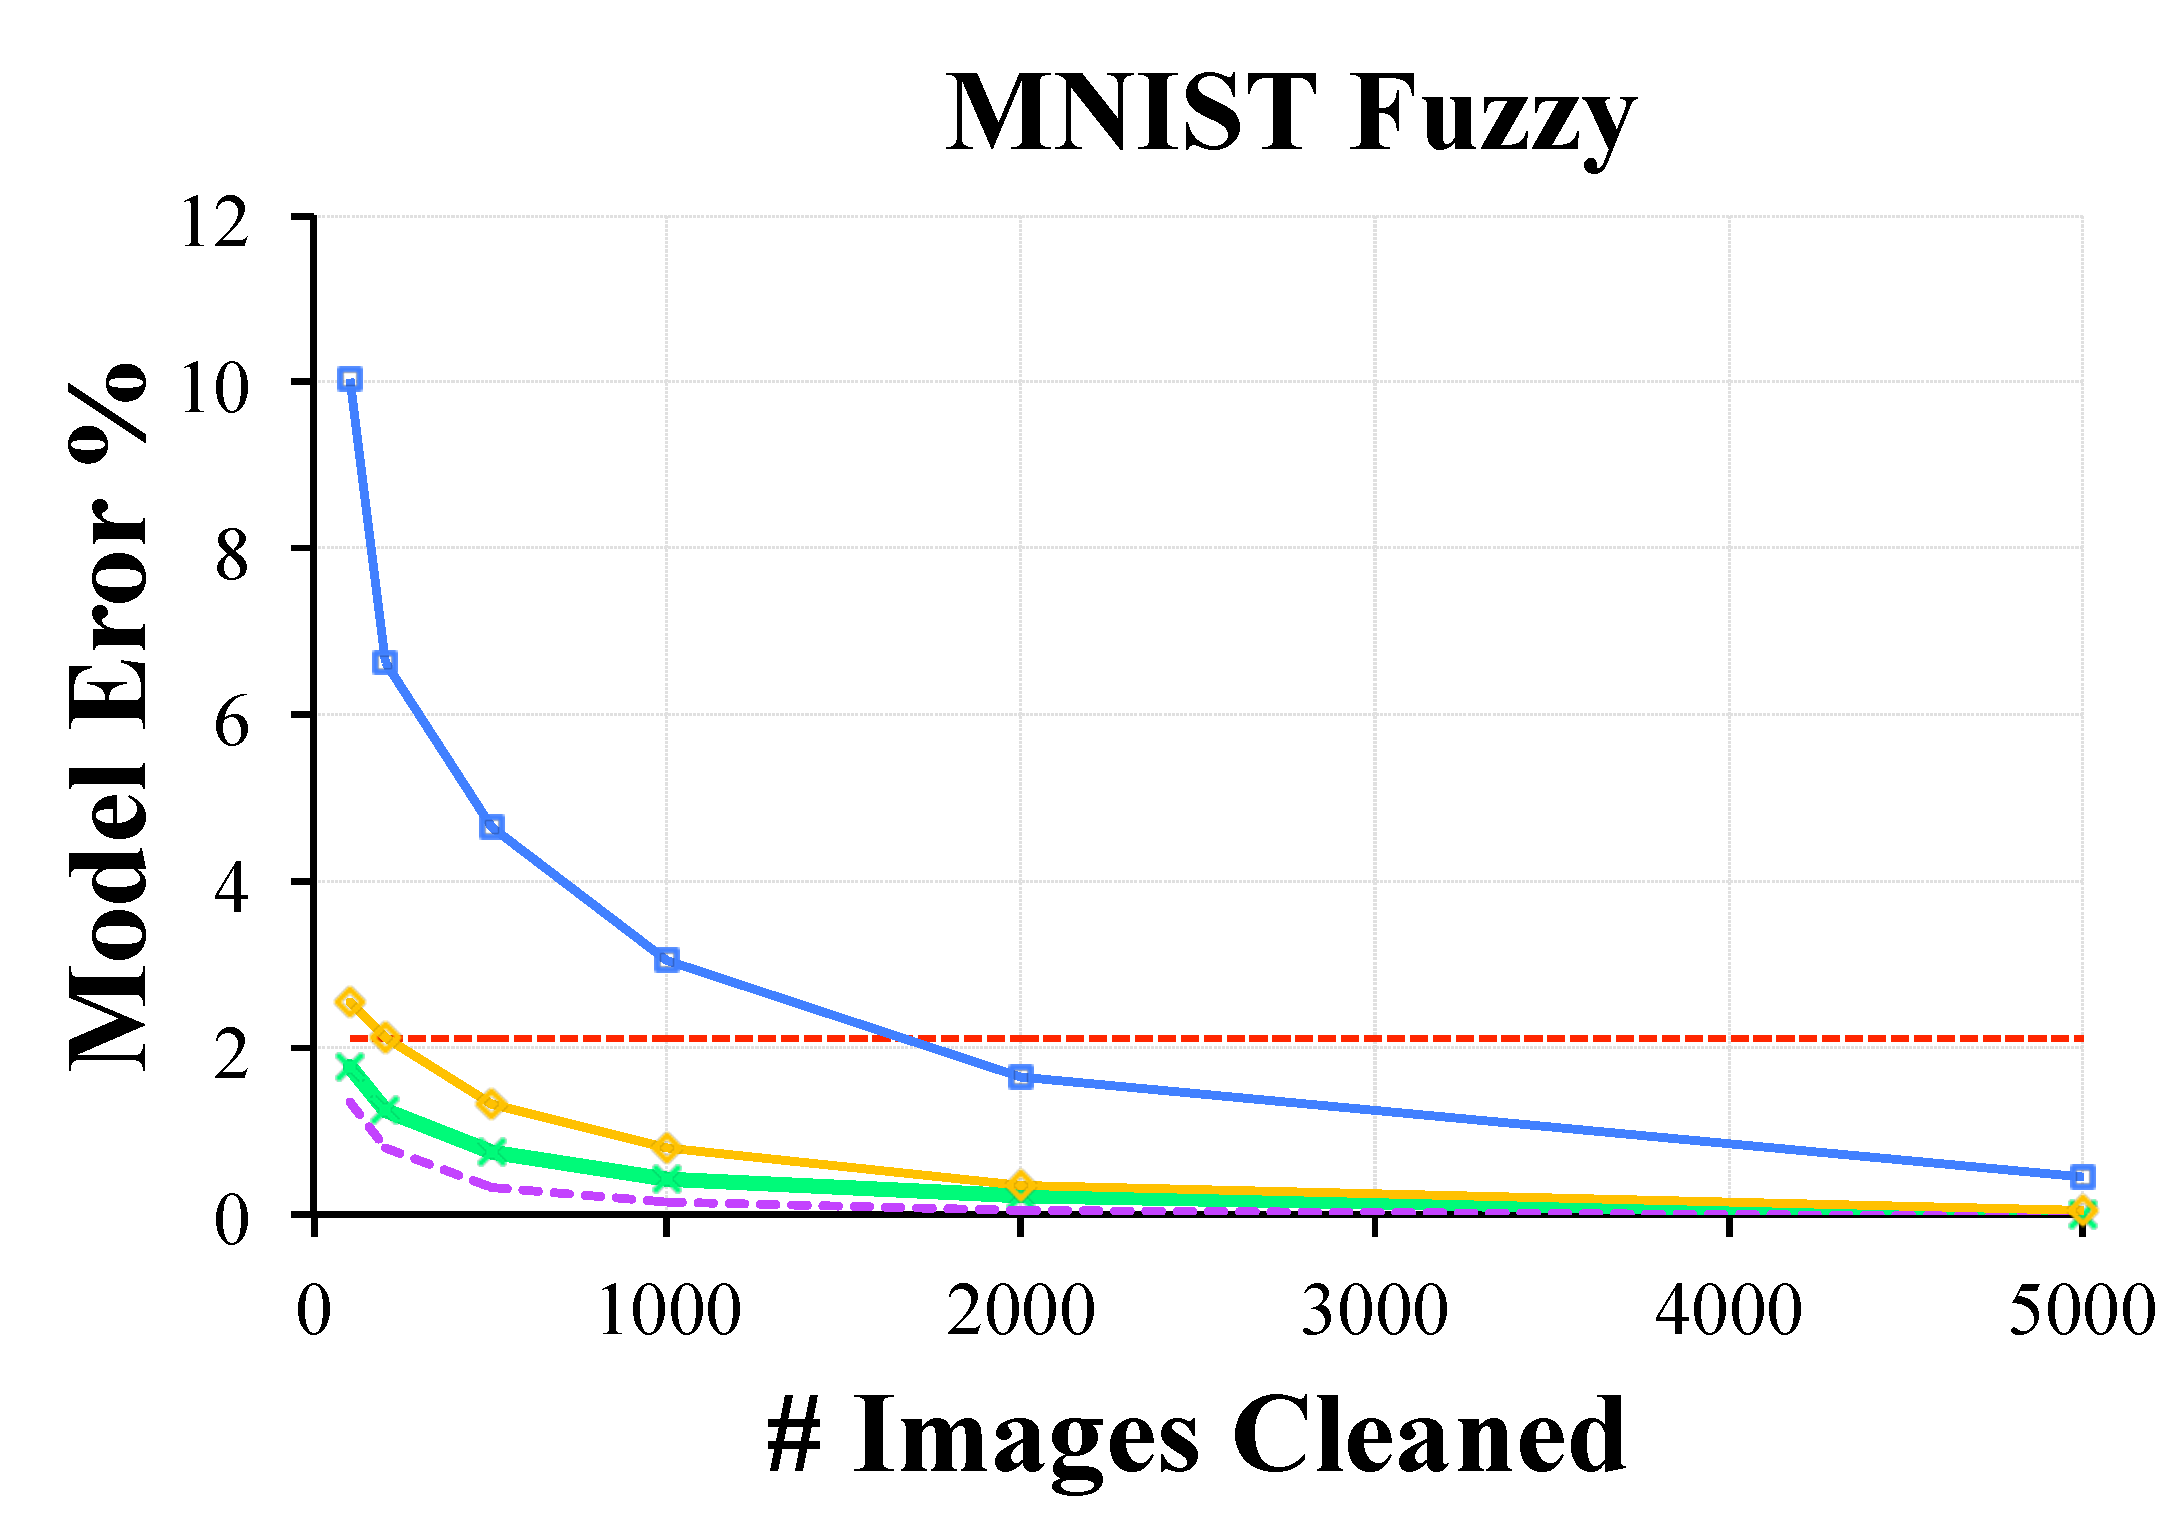
\includegraphics[scale=0.16]{exp/exp7b.pdf}
 \caption{For both types of corruption, \sys converges faster than Active Learning and SampleClean. \label{mnist}}
\end{figure}

\reminder{CFD: Adult}